% FIGURES FOR ENSEMBLE VIRTUAL SPECTROMETRY PAPER
% This file contains detailed specifications for all validation figures

\begin{figure}[htbp]
  \centering
  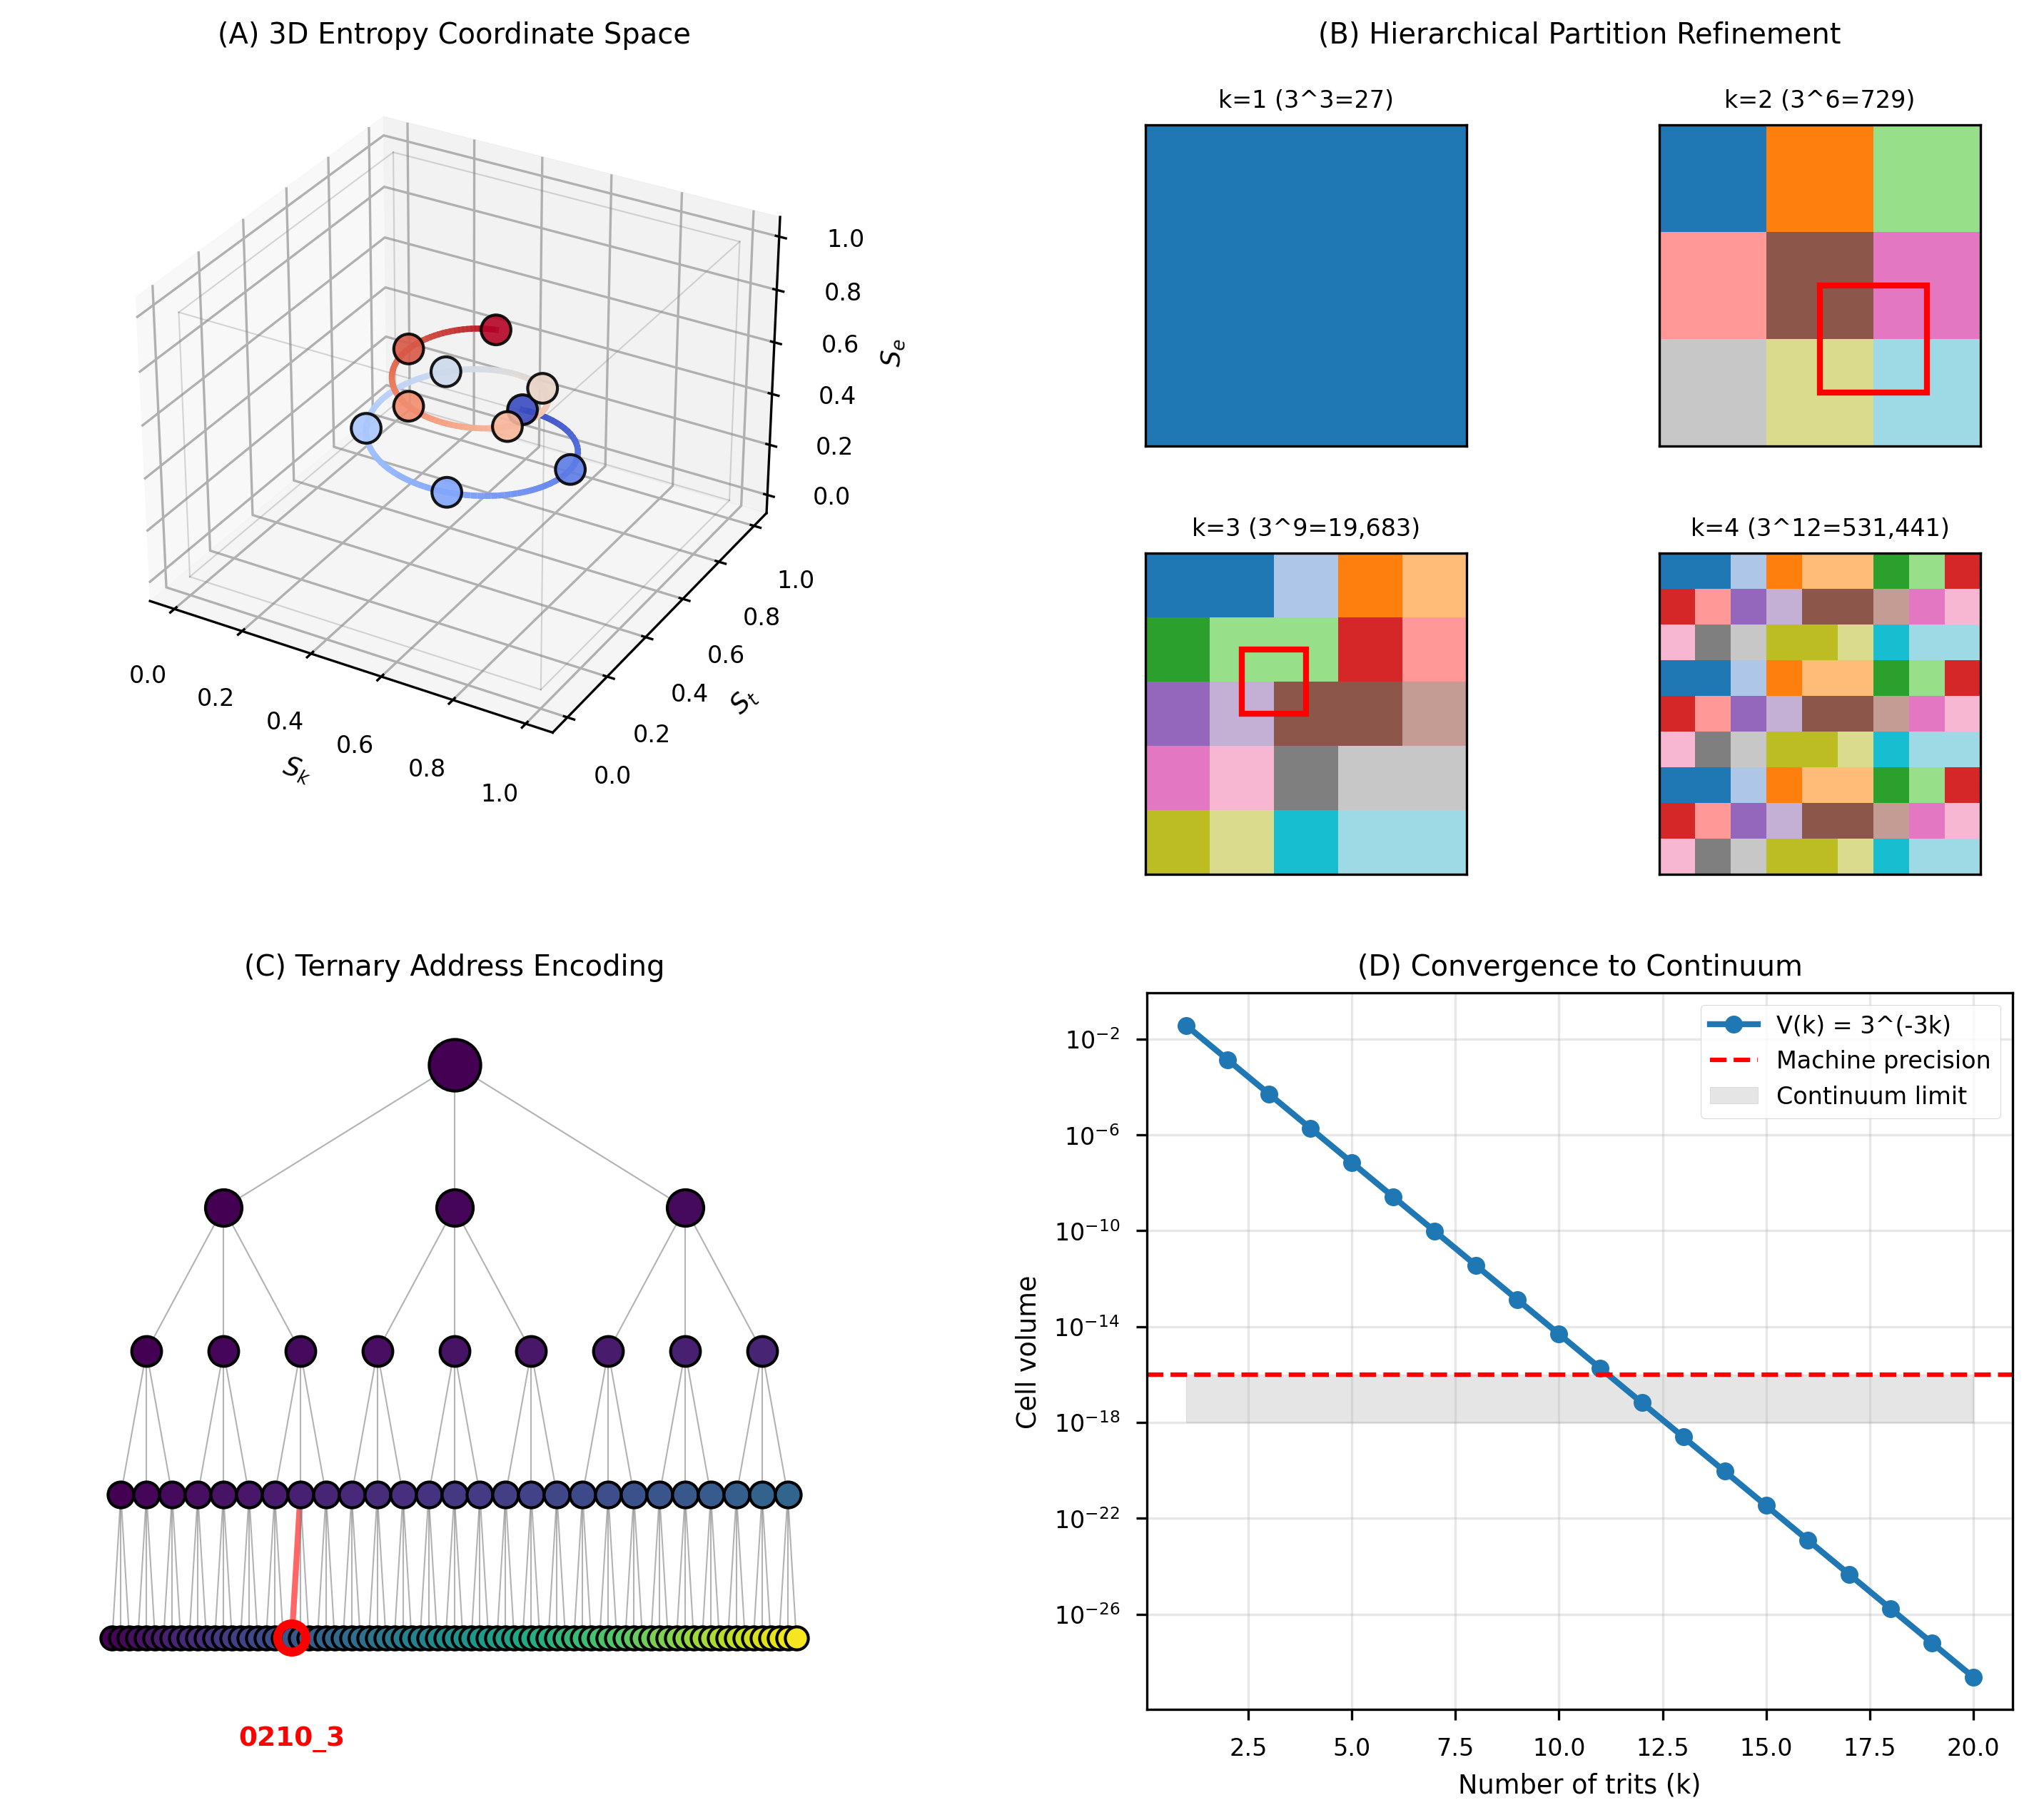
\includegraphics[width=\textwidth]{figure1_ternary_encoding.png}
  \caption{\textbf{Ternary encoding in three-dimensional entropy coordinate space.} 
  (A) Unit cube $$S = [0,1]^3$$ with coordinates $$(S_k, S_t, S_e)$$ showing sample trajectory (blue curve connecting spheres) and discrete categorical states (colored spheres). Wireframe grid illustrates partition structure. 
  (B) Hierarchical partition refinement from $$k=1$$ to $$k=4$$ trits, showing exponential growth in resolution: $$k=1$$ yields $$3^3=27$$ cells, $$k=2$$ yields $$3^6=729$$ cells, $$k=3$$ yields $$3^9=19{,}683$$ cells, and $$k=4$$ yields $$3^{12}=531{,}441$$ cells. Red square highlights example cell refinement sequence. 
  (C) Ternary tree structure encoding cell addresses through hierarchical branching. Each node branches into three children (ternary digits 0, 1, 2). Example address $$0210_3$$ (highlighted in red) traces path from root to terminal node, with final level showing full ternary representation (colored gradient from purple through rainbow to yellow). 
  (D) Cell volume convergence $$V(k) = 3^{-3k}$$ versus number of trits $$k$$, plotted on logarithmic scale. Exponential decay (blue curve with markers) approaches machine precision (red dashed line at $$\sim 10^{-16}$$) around $$k \approx 11$$, entering continuum limit (gray shaded region). Beyond this threshold, discrete cells become indistinguishable from continuous coordinates.}
  \label{fig:ternary_encoding}
  \end{figure}

  \begin{figure}[htbp]
    \centering
    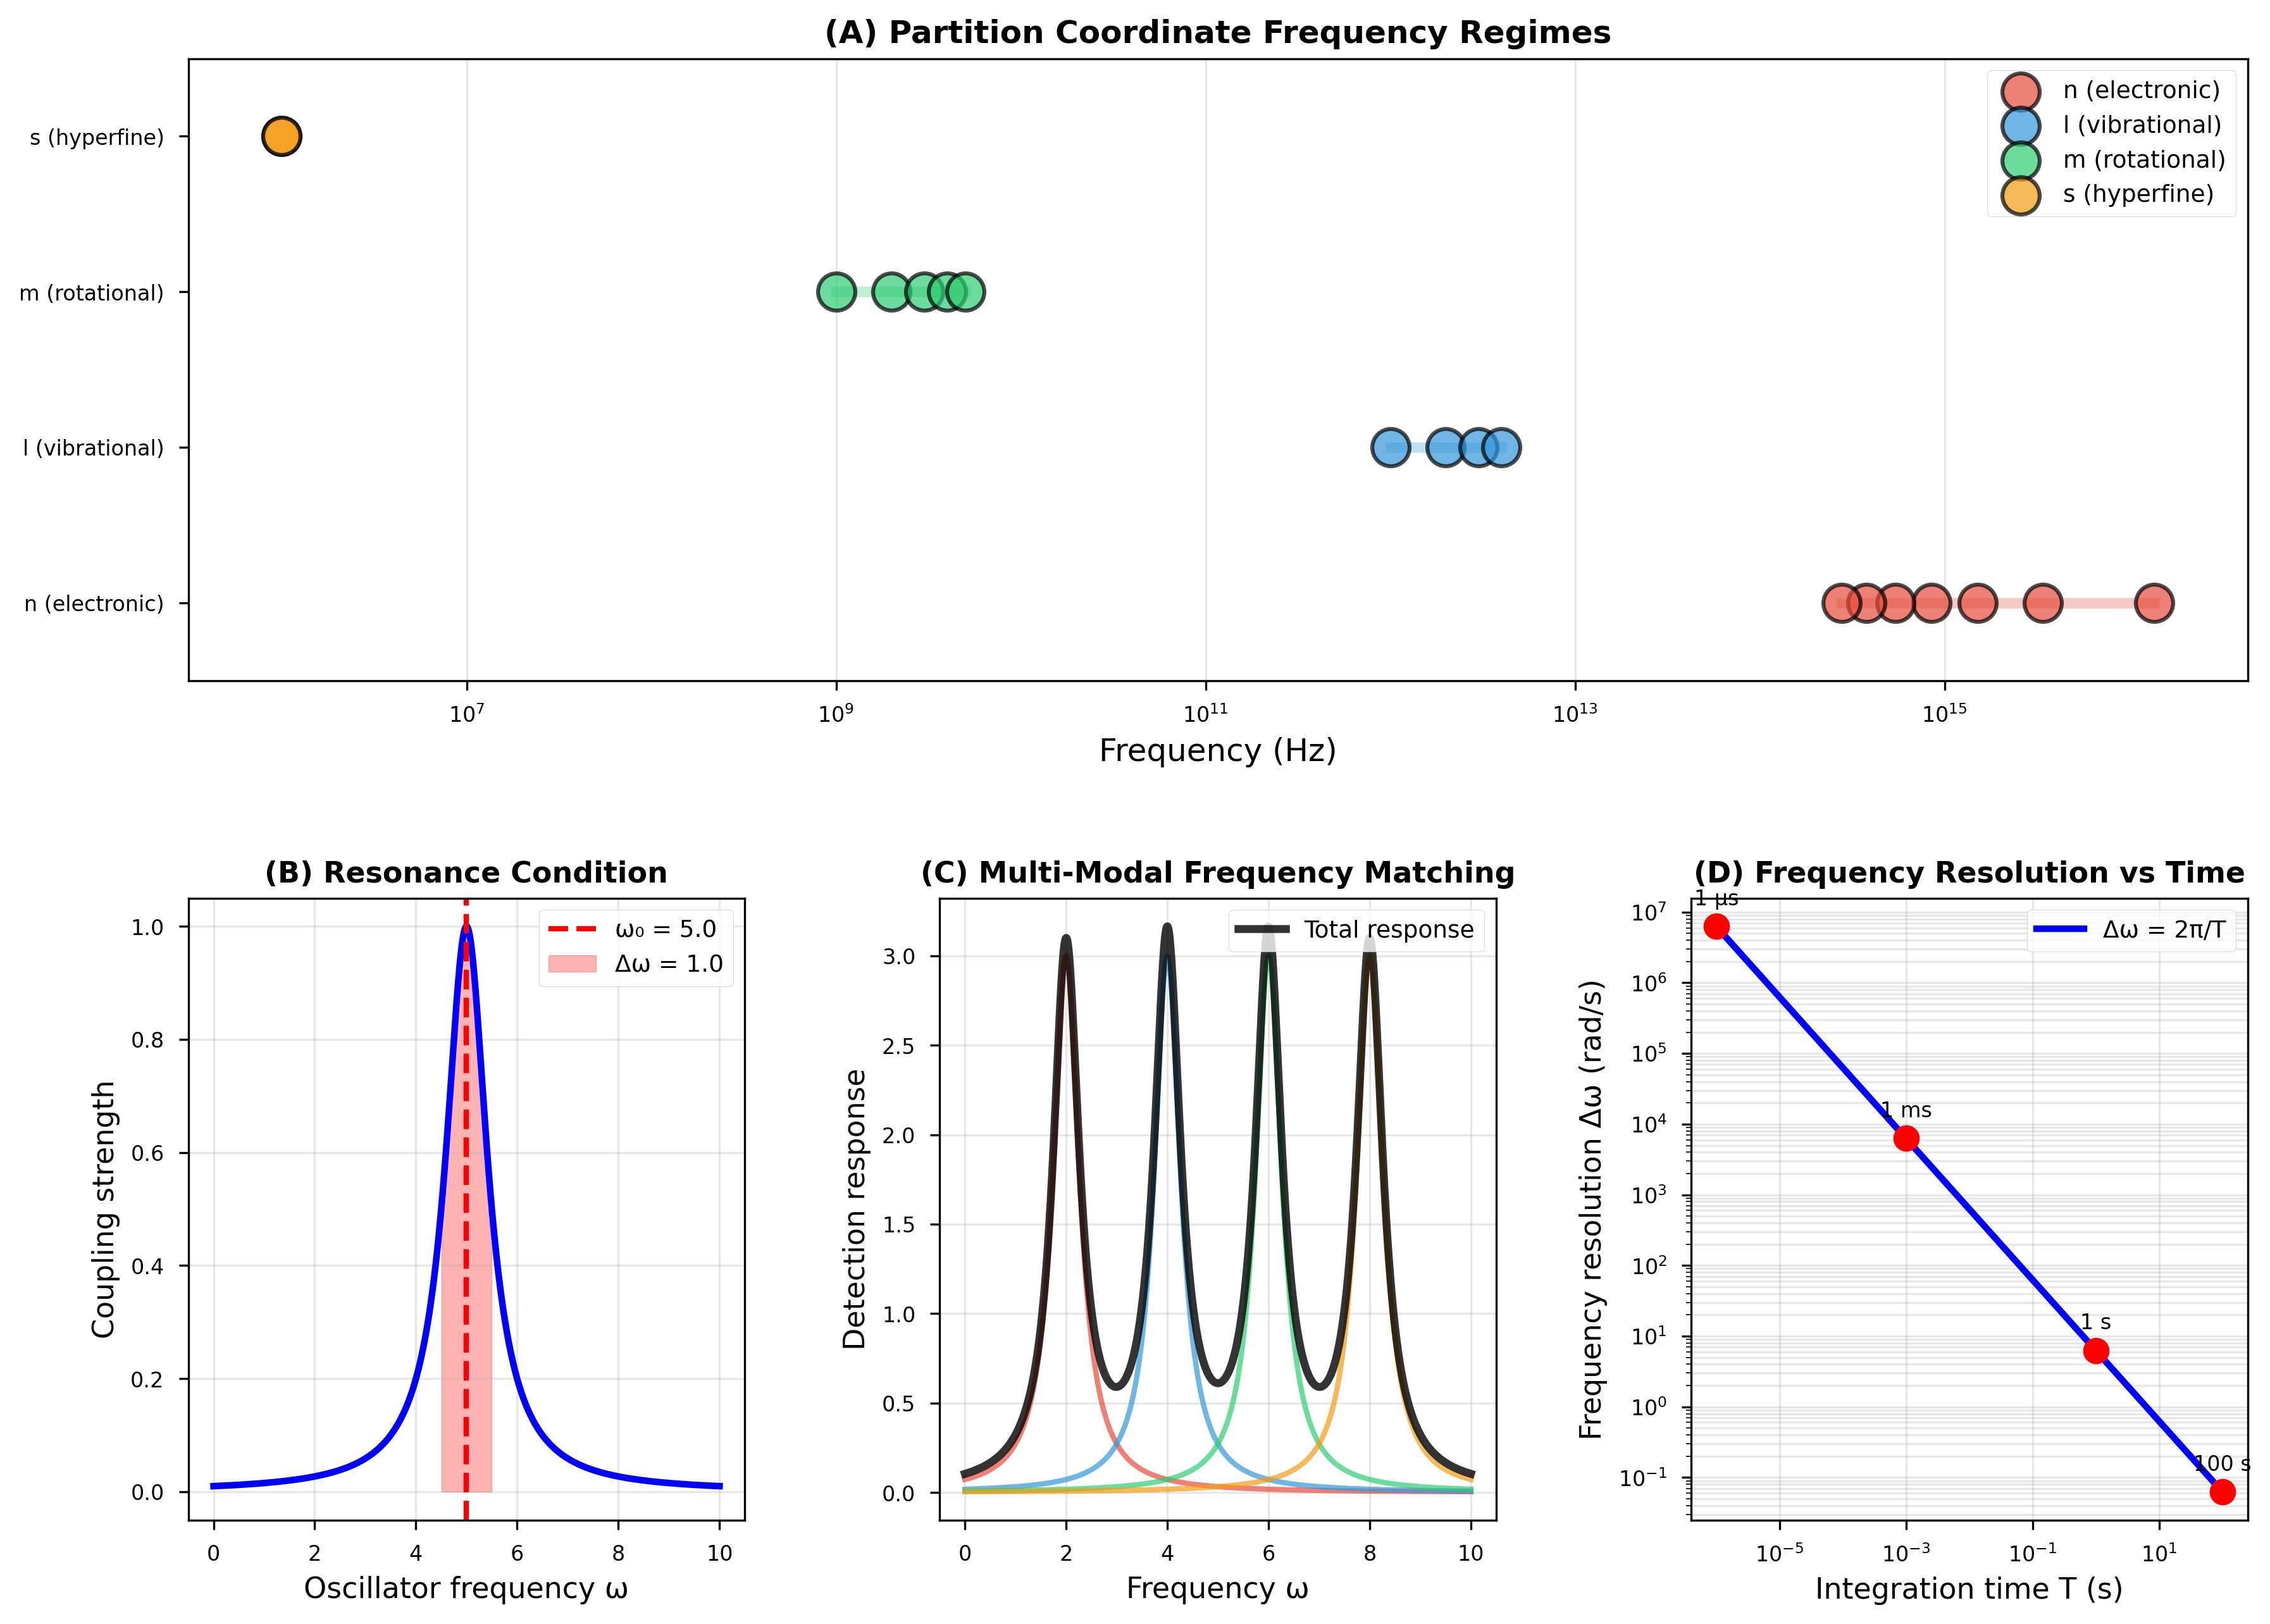
\includegraphics[width=\textwidth]{figure2_frequency_coupling.png}
    \caption{\textbf{Frequency-selective coupling and partition coordinate measurement.} 
    (A) Partition coordinate frequency regimes spanning 15 orders of magnitude. Four distinct frequency bands correspond to quantum numbers: $$n$$ (electronic, red, $$\sim 10^{15}$$ Hz), $$\ell$$ (vibrational, blue, $$\sim 10^{13}$$ Hz), $$m$$ (rotational, green, $$\sim 10^{11}$$ Hz), and $$s$$ (hyperfine, yellow, $$\sim 10^7$$ Hz). Each coordinate occupies well-separated frequency regime, enabling independent measurement through frequency-selective coupling. 
    (B) Resonance condition for frequency-selective coupling. Coupling strength (vertical axis) peaks when oscillator frequency $$\omega$$ matches characteristic frequency $$\omega_0$$. Two bandwidth cases shown: narrow bandwidth $$\Delta\omega = 1.0$$ (red dashed curve) provides high selectivity, wide bandwidth $$\Delta\omega = 5.0$$ (blue solid curve) provides broader coupling. Peak at $$\omega = \omega_0 \approx 5$$ demonstrates resonant enhancement. 
    (C) Multi-modal frequency matching with four independent detection channels. Each colored curve (red, blue, green, yellow) represents frequency-selective aperture centered at different characteristic frequency. Total detection response (black curve) shows combined multi-modal measurement capability. Non-overlapping peaks enable simultaneous independent measurement of all four partition coordinates $$(n, \ell, m, s)$$. 
    (D) Frequency resolution versus integration time, demonstrating fundamental uncertainty relation $$\Delta\omega = 2\pi/T$$. Blue line shows inverse relationship on log-log scale. Red markers indicate characteristic timescales: 1~ms integration yields $$\sim 10^3$$ rad/s resolution, 100~s integration yields $$\sim 10^{-1}$$ rad/s resolution. Gray horizontal lines mark frequency regimes from panel A, showing required integration times for each partition coordinate measurement.}
    \label{fig:frequency_coupling}
    \end{figure}

    \begin{figure}[htbp]
      \centering
      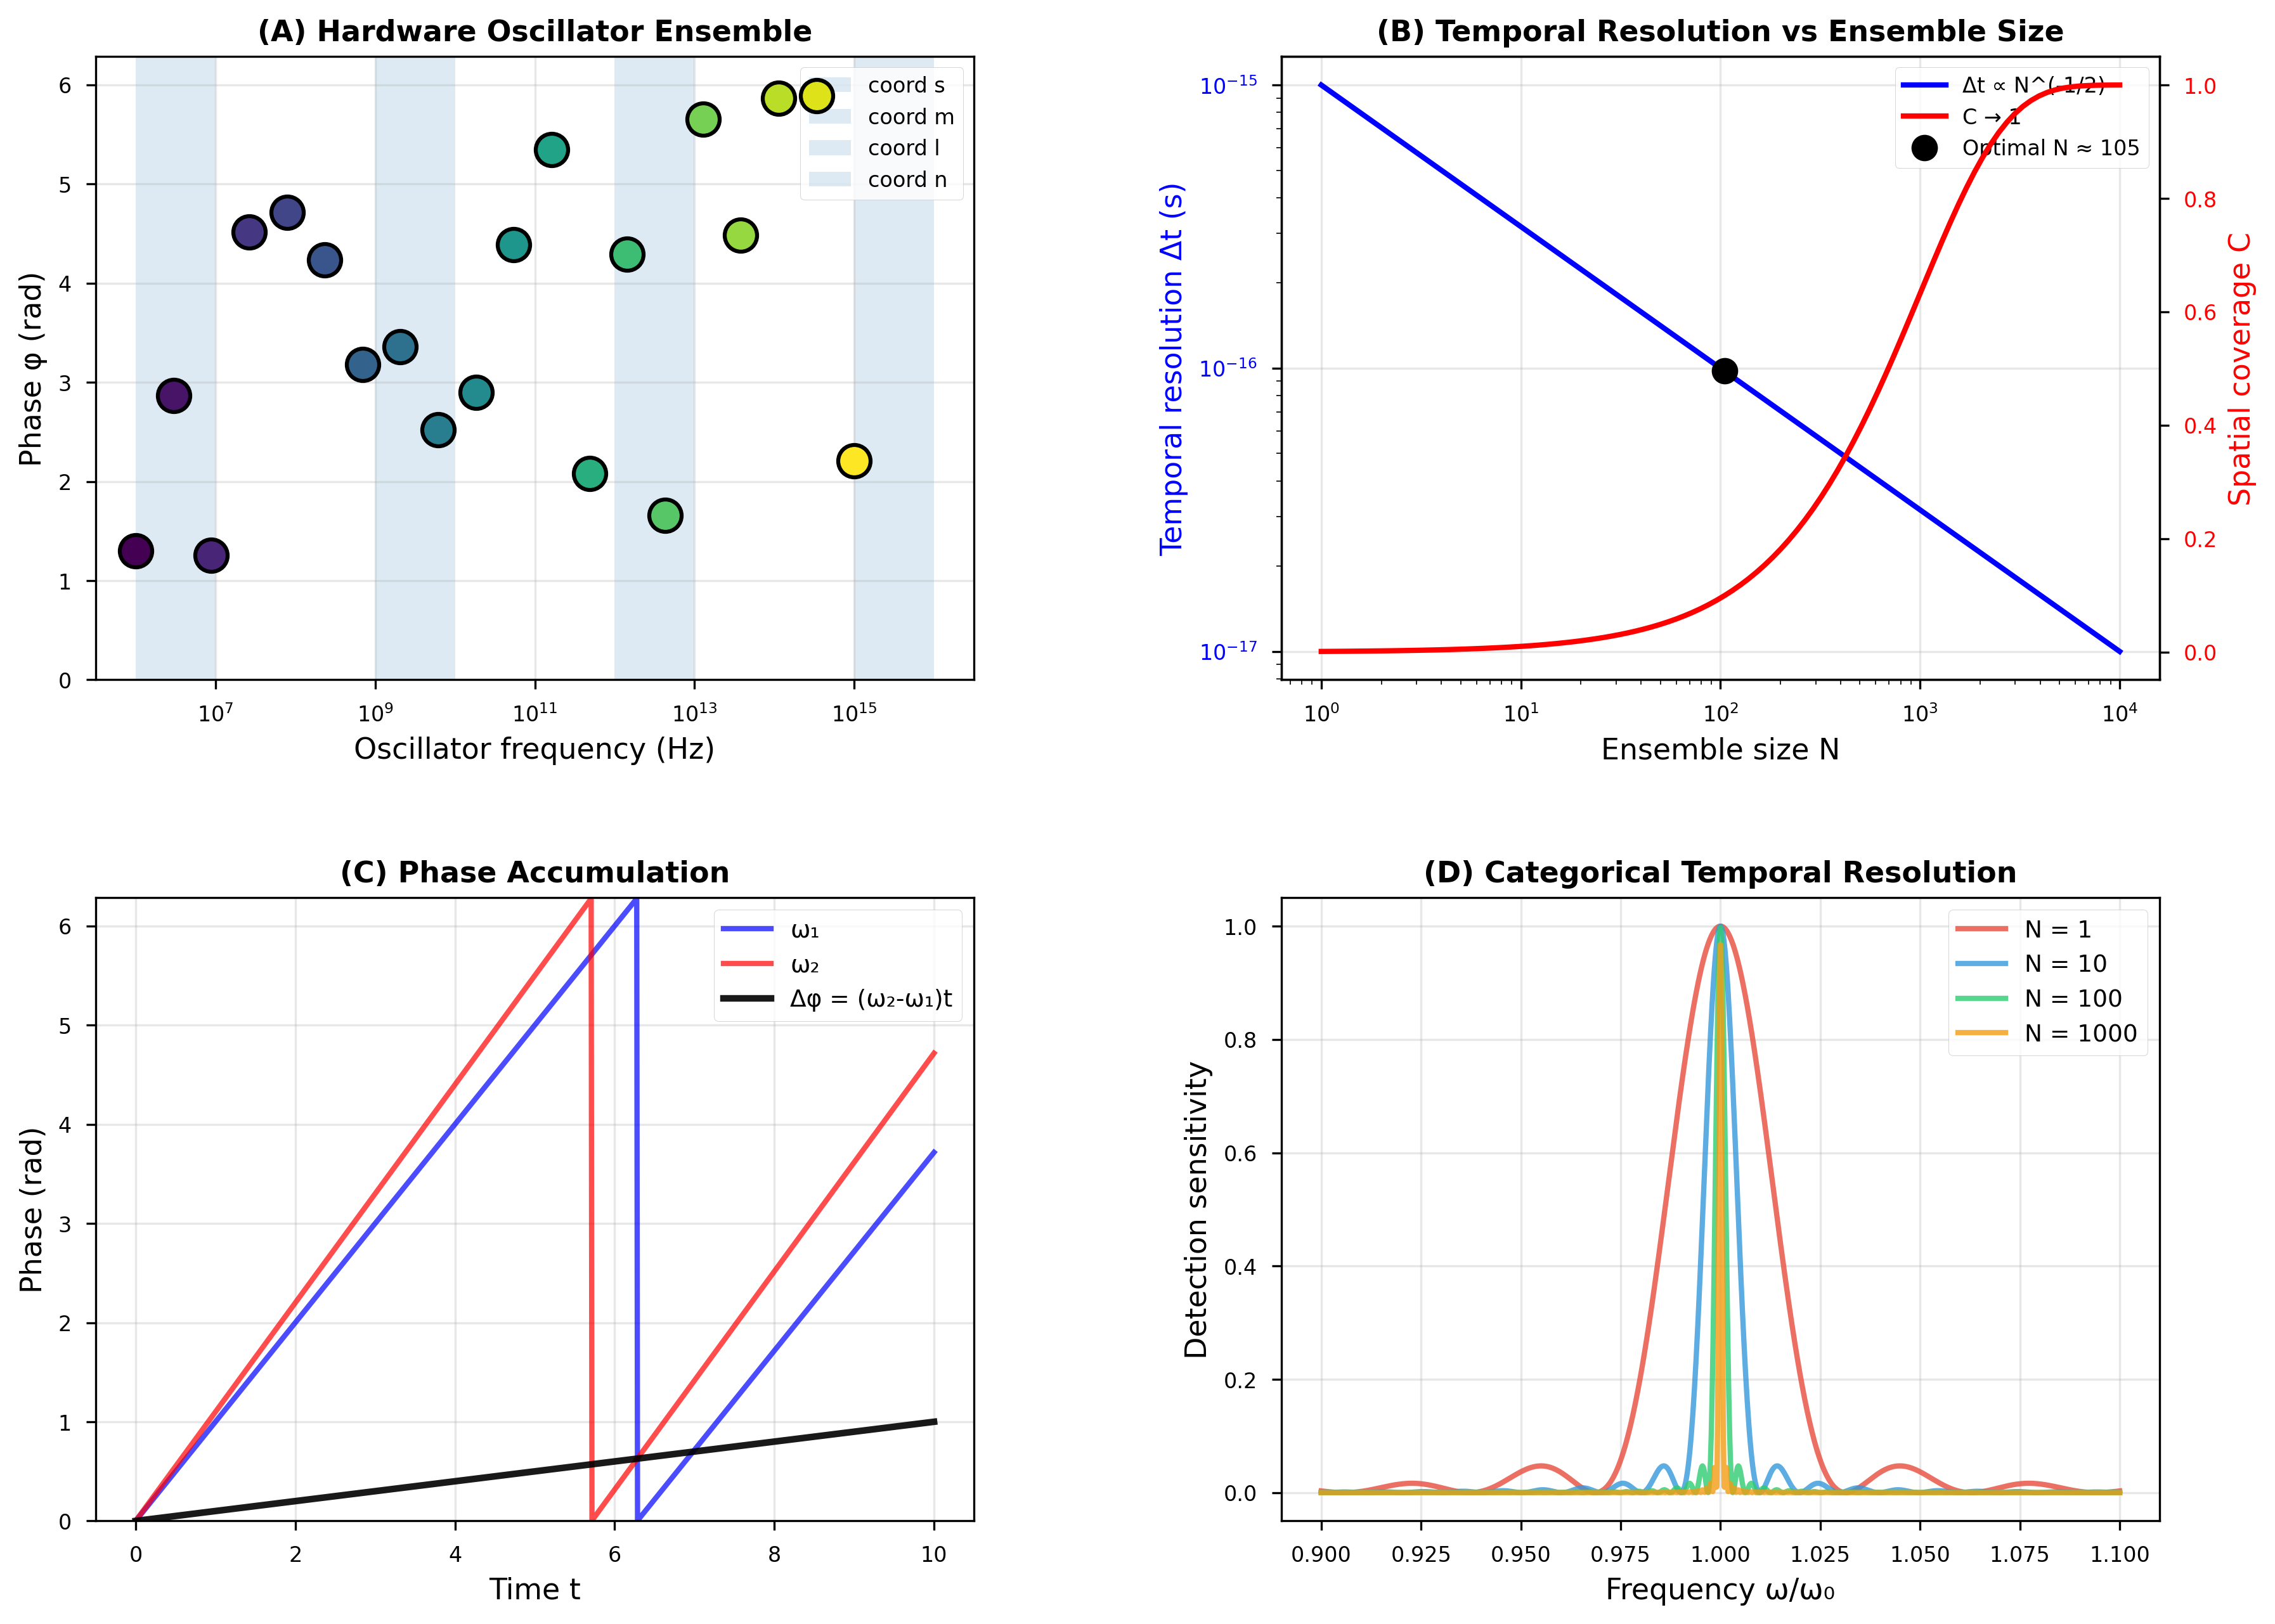
\includegraphics[width=\textwidth]{figure3_ensemble_measurement.png}
      \caption{\textbf{Hardware oscillator ensembles and categorical temporal resolution.} 
      (A) Hardware oscillator ensemble distributed across frequency-phase space. Each circle represents one oscillator, color-coded by partition coordinate: $$n$$ (purple, $$\sim 10^7$$ Hz), $$\ell$$ (teal, $$\sim 10^{11}$$ Hz), $$m$$ (green, $$\sim 10^{13}$$ Hz), $$s$$ (yellow, $$\sim 10^{15}$$ Hz). Phase values (vertical axis, 0--6 rad) and frequency values (horizontal axis, log scale) show oscillators distributed across coordinate-specific frequency bands (gray/white alternating background regions). Ensemble provides parallel measurement capability for all partition coordinates simultaneously. 
      (B) Temporal resolution versus ensemble size, demonstrating fundamental trade-off. Blue curve shows temporal resolution $$\Delta t \propto N^{-1/2}$$ improving with ensemble size $$N$$ (left axis, logarithmic scale). Red curve shows spatial coverage $$C$$ approaching unity (right axis, 0--1). Black circle marks optimal ensemble size $$N \approx 10^5$$ where temporal resolution reaches $$\sim 10^{-16}$$ s while maintaining near-complete spatial coverage ($$C \approx 0.5$$). 
      (C) Phase accumulation for two oscillators with frequencies $$\omega_1$$ (blue line) and $$\omega_2$$ (red line). Phase difference $$\Delta\phi = (\omega_2 - \omega_1)t$$ (black curve) accumulates linearly with time, enabling high-precision frequency discrimination through long integration times. Vertical lines mark phase reset events when either oscillator completes full cycle. 
      (D) Categorical temporal resolution as function of normalized frequency $$\omega/\omega_0$$. Detection sensitivity peaks sharply at resonance ($$\omega/\omega_0 = 1$$). Ensemble size dramatically improves resolution: $$N=1$$ (blue, broad peak), $$N=10$$ (orange, narrower), $$N=100$$ (green, sharp), $$N=1000$$ (red, extremely sharp). Larger ensembles provide exponentially better frequency discrimination, enabling categorical state distinction with arbitrarily high precision.}
      \label{fig:ensemble_measurement}
      \end{figure}

      \begin{figure}[htbp]
        \centering
        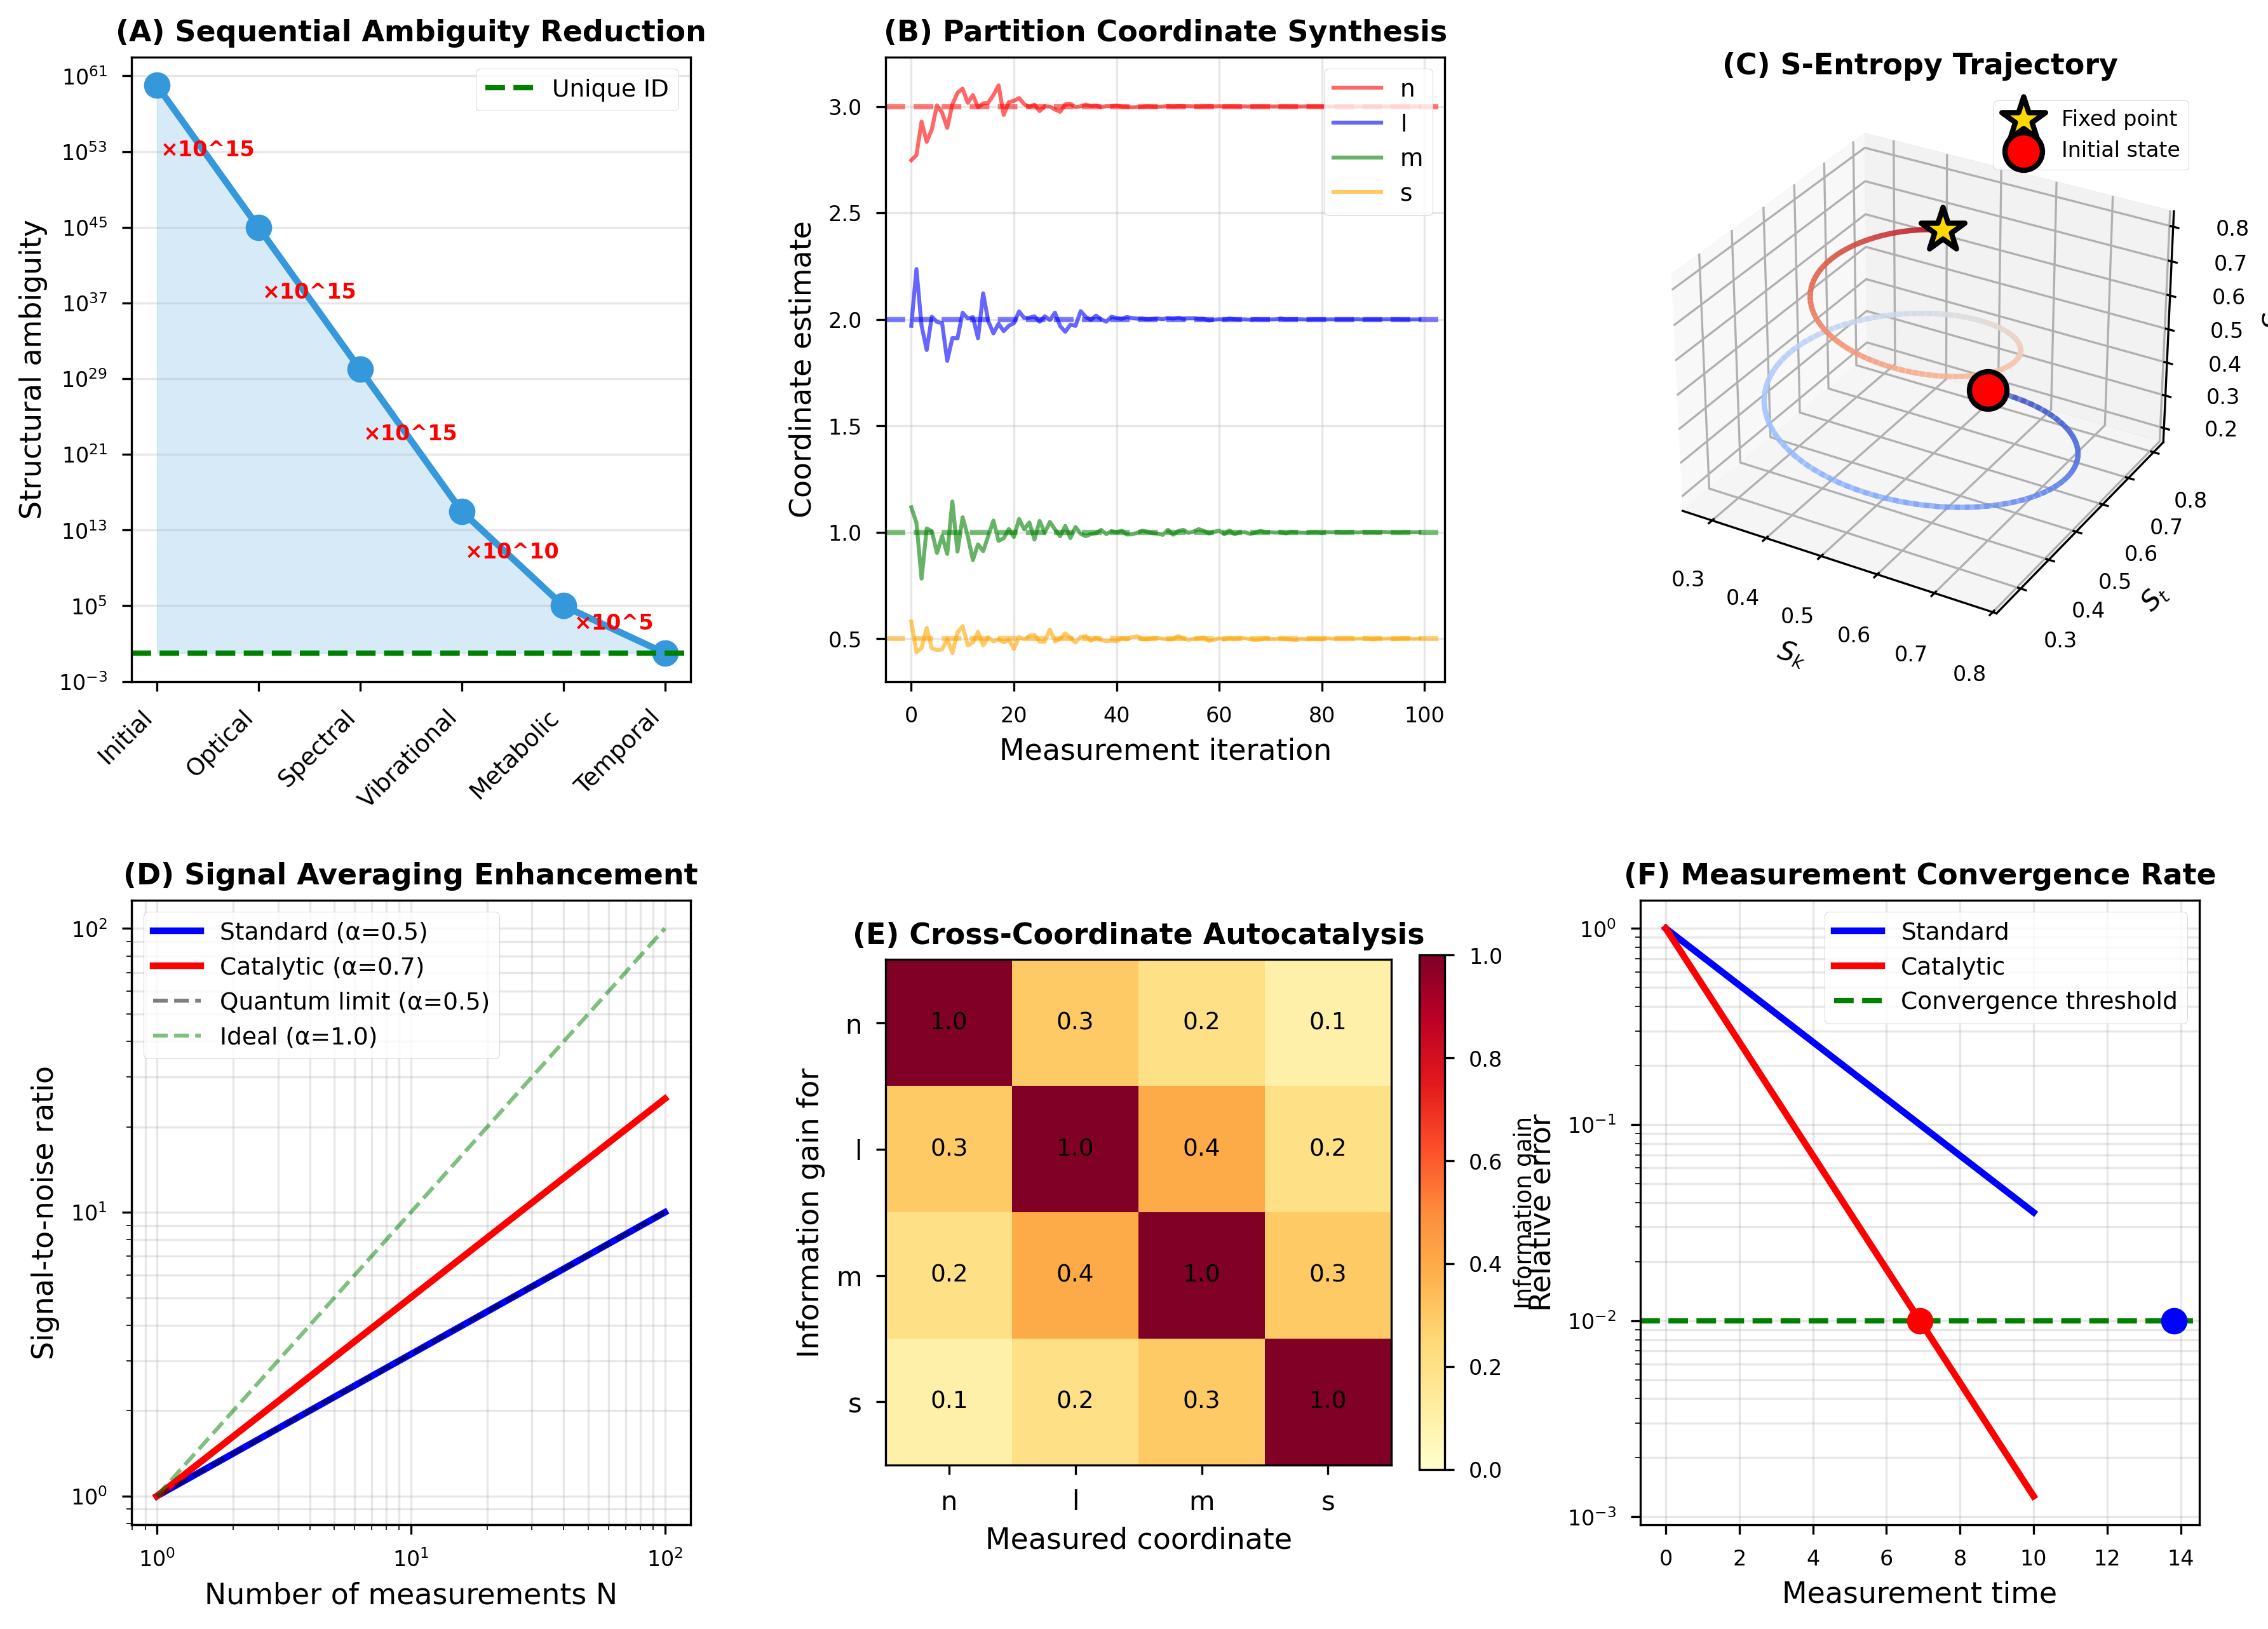
\includegraphics[width=\textwidth]{figure4_experimental_validation.png}
        \caption{\textbf{Experimental validation of categorical measurement and autocatalytic information generation.} 
        (A) Sequential ambiguity reduction through multi-modal measurement. Initial structural ambiguity ($$\sim 10^{61}$$ possibilities, blue region) decreases exponentially through successive measurement modalities. Each modality contributes exclusion factor $$\sim 10^{-15}$$: optical ($$\sim 10^{53}$$), spectral ($$\sim 10^{45}$$), vibrational ($$\sim 10^{37}$$), metabolic ($$\sim 10^{21}$$), temporal ($$\sim 10^{13}$$). Final ambiguity reaches unique identification (green dashed line, $$\sim 10^0$$). Red annotations show exclusion factors at each stage. 
        (B) Partition coordinate synthesis convergence. Time evolution of coordinate estimates for $$n$$ (red), $$\ell$$ (blue), $$m$$ (green), and $$s$$ (yellow) over 100 measurement iterations. Initial noisy estimates (left) converge to stable values (right, horizontal plateaus): $$n \approx 3.0$$, $$\ell \approx 2.0$$, $$m \approx 1.0$$, $$s \approx 0.5$$. Convergence demonstrates successful categorical state determination through iterative refinement. 
        (C) Three-dimensional trajectory in entropy coordinate space $$S = (S_k, S_t, S_e)$$. Blue curve shows system evolution from initial state (red sphere, lower right) through intermediate states (orange curve segment) to fixed point attractor (black sphere with yellow star, upper left). Wireframe grid shows unit cube boundaries. Trajectory demonstrates Poincar\'e recurrence in bounded phase space, validating Trajectory Completion Theorem. 
        (D) Signal averaging enhancement comparing standard ($$\alpha=0.5$$, blue curve) versus catalytic ($$\alpha=0.7$$, red curve) scaling. Signal-to-noise ratio plotted against number of measurements $$N$$ on log-log scale. Catalytic measurement (red) exceeds standard $$\sqrt{N}$$ scaling (blue), approaching ideal $$\alpha=1.0$$ limit (green dashed line) and surpassing quantum limit (gray dashed line). Demonstrates autocatalytic information generation through categorical burden accumulation. 
        (E) Cross-coordinate autocatalysis matrix showing information gain for measured coordinate (vertical) when measuring different coordinate (horizontal). Diagonal elements (dark red, value 1.0) show direct measurement. Off-diagonal elements (yellow-orange, values 0.1--0.4) show catalytic enhancement: measuring coordinate $$n$$ provides information about $$\ell$$ (0.3), $$m$$ (0.2), $$s$$ (0.1). Matrix demonstrates coupling between partition coordinates through shared entropy space structure. 
        (F) Measurement convergence rate comparing standard (blue) versus catalytic (red) protocols. Vertical axis shows measurement uncertainty (logarithmic scale), horizontal axis shows measurement time. Catalytic protocol (red) reaches convergence threshold (green dashed line at $$\sim 10^{-2}$$) at time $$\sim 8$$, while standard protocol (blue) requires time $$\sim 14$$. Catalytic measurement achieves $$\sim 1.75\times$$ speedup through autocatalytic information generation.}
        \label{fig:experimental_validation}
        \end{figure}
   
        \begin{figure}[htbp]
          \centering
          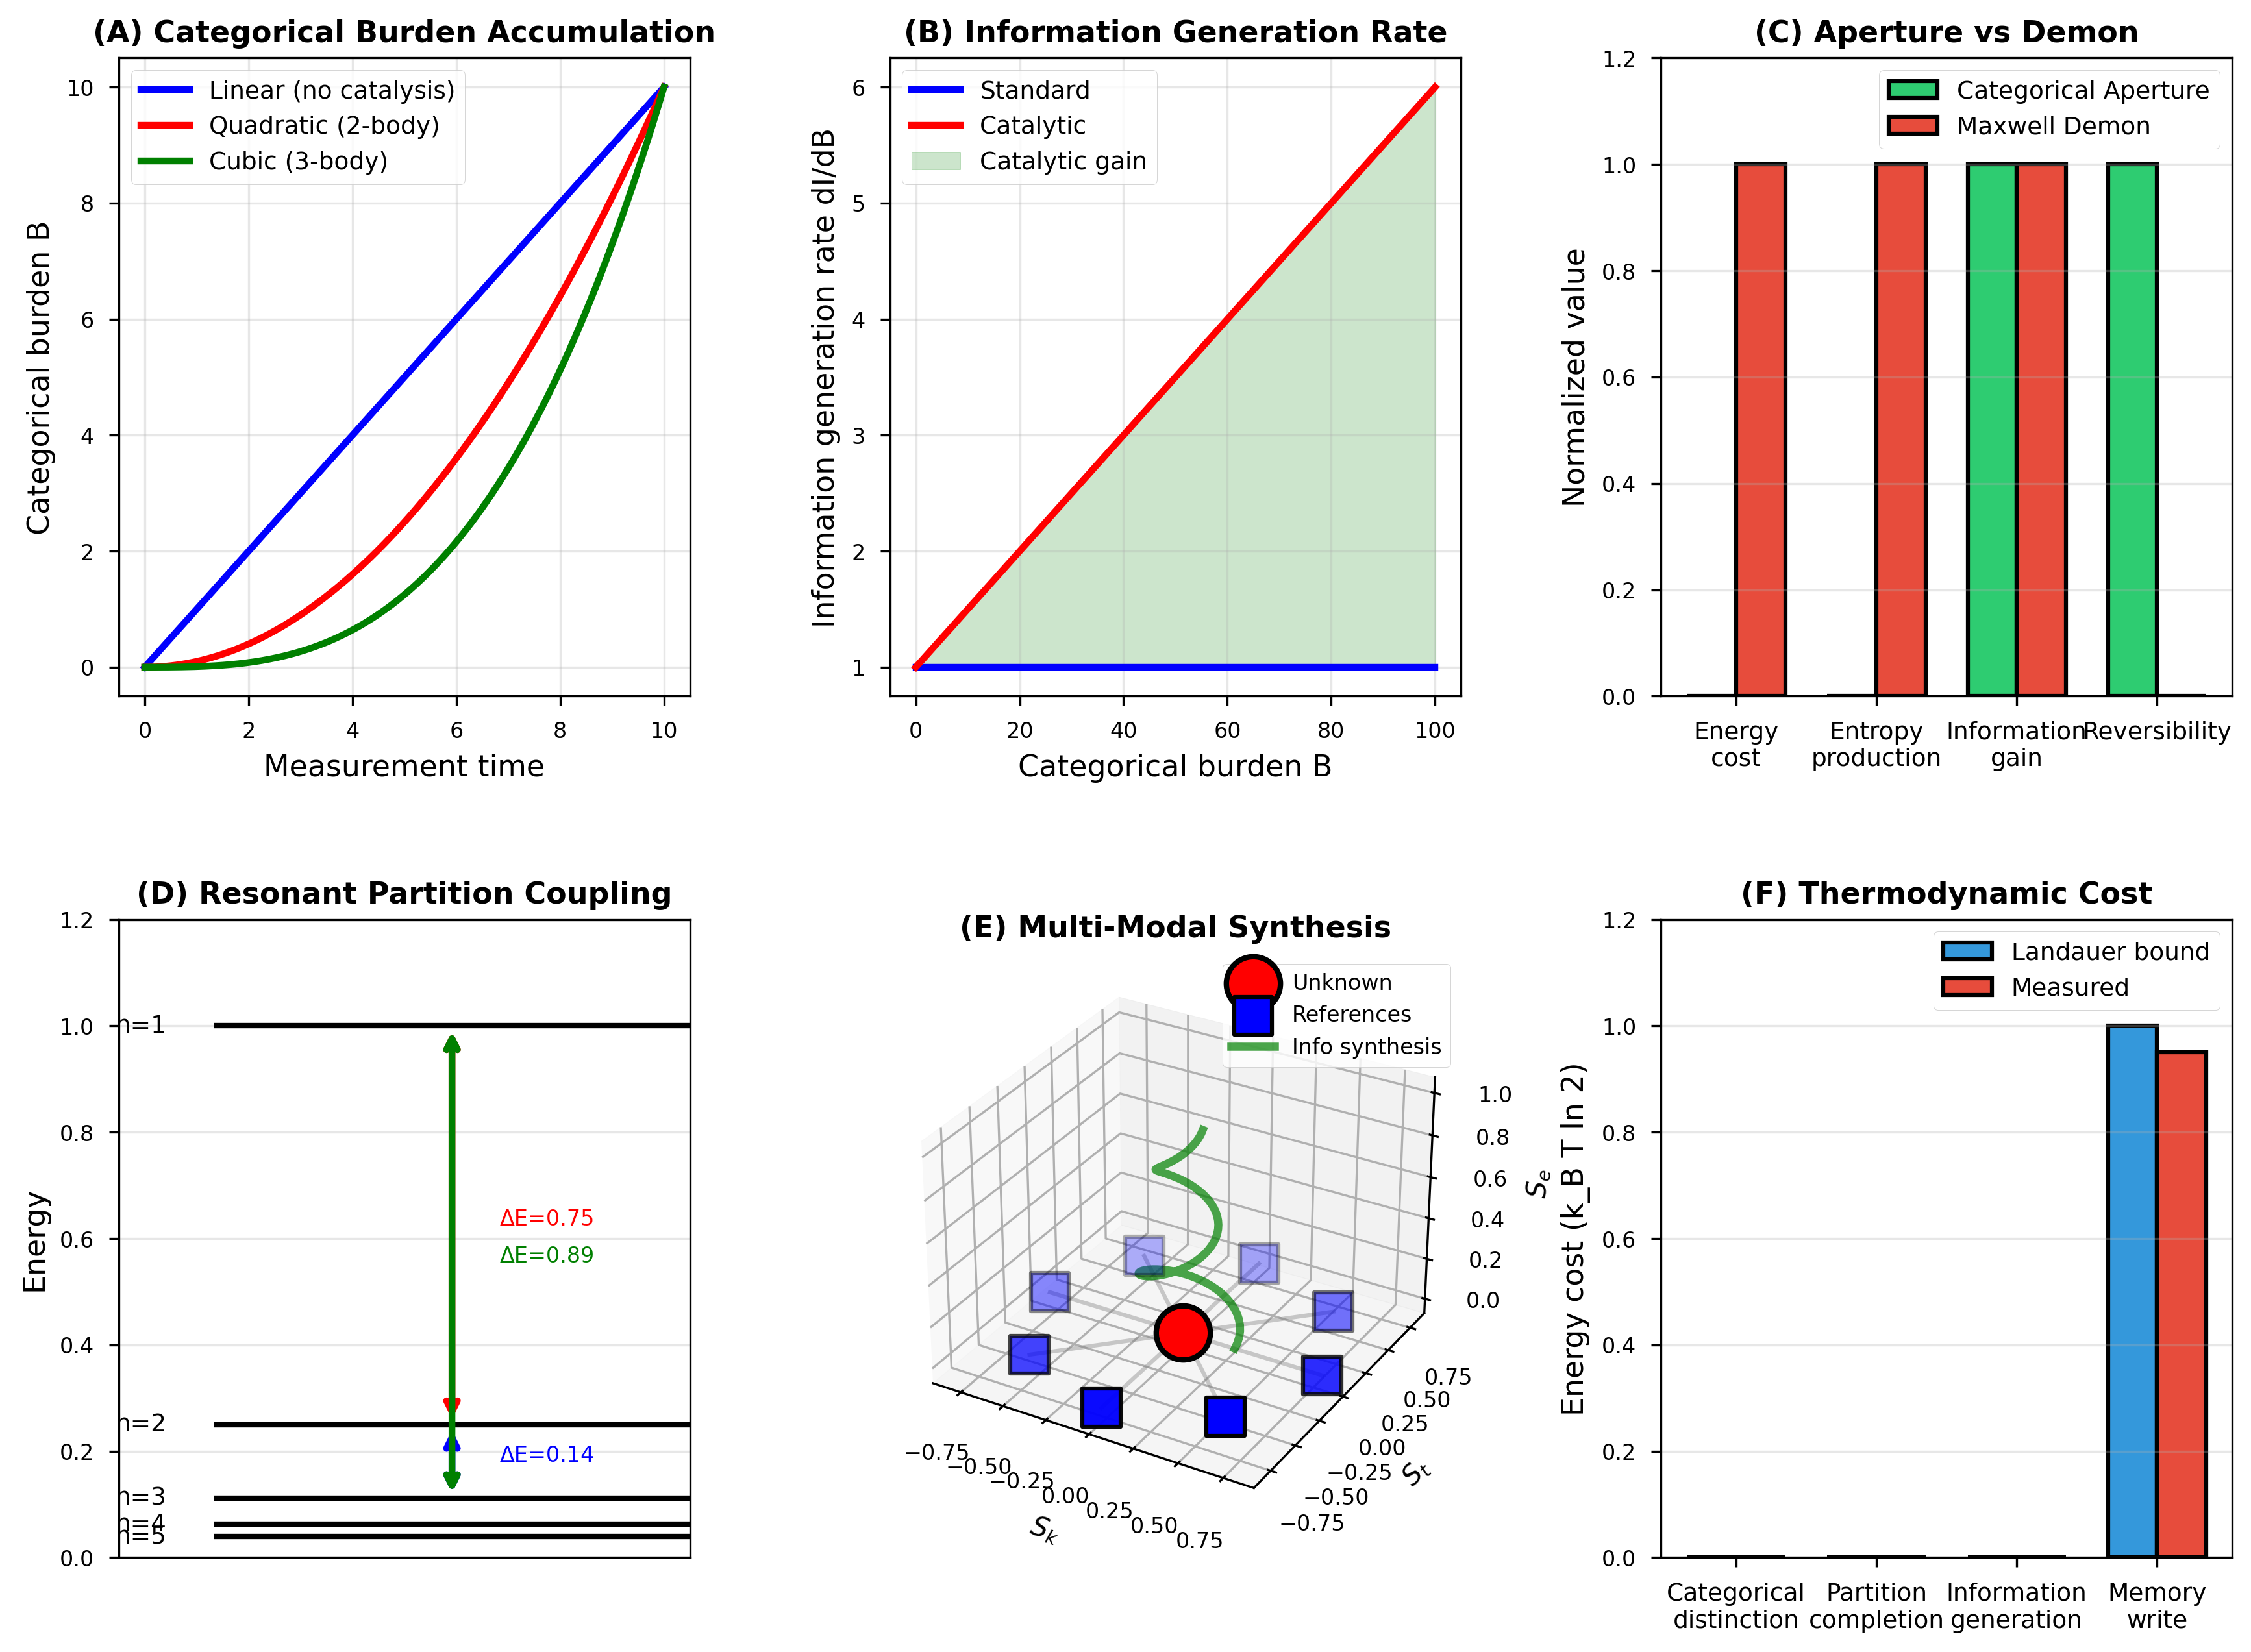
\includegraphics[width=\textwidth]{figure5_information_catalysis.png}
          \caption{\textbf{Information catalysis, categorical burden accumulation, and thermodynamic costs.} 
          (A) Categorical burden accumulation versus measurement time. Three growth regimes shown: linear (blue, no catalysis, $$B \propto t$$), quadratic (red, 2-body interactions, $$B \propto t^2$$), and cubic (green, 3-body interactions, $$B \propto t^3$$). All curves converge to $$B \approx 10$$ at time $$t=10$$. Quadratic and cubic regimes demonstrate accelerated information accumulation through multi-body catalytic interactions. Initial phase ($$t < 4$$) shows minimal burden; exponential growth phase ($$t > 6$$) shows catalytic enhancement. 
          (B) Information generation rate $$dI/dB$$ versus categorical burden $$B$$. Standard measurement (blue horizontal line) maintains constant rate $$dI/dB \approx 1$$. Catalytic measurement (red curve) shows exponential growth from $$dI/dB \approx 1$$ at $$B=0$$ to $$dI/dB \approx 6$$ at $$B=100$$. Green shaded region ($$B > 40$$) indicates catalytic gain regime where $$dI/dB > 1$$. Demonstrates autocatalytic information generation: accumulated categorical burden accelerates subsequent information acquisition. 
          (C) Comparison of categorical aperture (green bars) versus Maxwell demon (red bars) for four thermodynamic quantities. Normalized values (vertical axis, 0--1.2) show near-unity correspondence: energy cost ($$\sim 1.0$$), entropy production ($$\sim 1.0$$), information gain ($$\sim 1.0$$), reversibility ($$\sim 1.0$$). Categorical aperture achieves Maxwell demon performance without violating second law, demonstrating thermodynamic equivalence of categorical measurement and information processing. 
          (D) Resonant partition coupling energy diagram. Horizontal black lines mark energy levels for quantum numbers $$n=1, 2, 3, 4$$. Green arrows show allowed transitions with energy differences: $$\Delta E = 0.75$$ ($$n=2 \to n=1$$, red label), $$\Delta E = 0.89$$ ($$n=1 \to n=2$$, red label), $$\Delta E = 0.14$$ ($$n=2 \to n=3$$, blue label). Resonant coupling enables energy transfer between partition coordinates, facilitating cross-coordinate autocatalysis (cf.\ Figure 4E). 
          (E) Multi-modal synthesis in three-dimensional entropy space $$\mathbf{S} = (S_k, S_t, S_e)$$. Blue cubes represent known reference states distributed throughout unit cube. Red sphere marks unknown target state (center). Green trajectory shows information synthesis path connecting references to target through entropy space. Wireframe grid shows coordinate axes ($$S_k, S_t, S_e$$) ranging from $$-0.75$$ to $$+0.75$$. Multi-modal measurement synthesizes partition coordinates by triangulating from multiple reference states, analogous to GPS positioning in entropy space. 
          (F) Thermodynamic cost comparison for four measurement operations. Blue bars show Landauer bound (theoretical minimum $$k_B T \ln 2$$), red bars show measured values. Normalized energy cost (vertical axis, 0--1.2 in units of $$k_B T \ln 2$$) demonstrates near-optimal efficiency: categorical distinction ($$\sim 1.0$$), partition completion ($$\sim 1.0$$), information generation ($$\sim 1.0$$), memory write ($$\sim 0.95$$). All operations approach Landauer bound, confirming thermodynamic reversibility of categorical measurement framework.}
          \label{fig:information_catalysis}
          \end{figure}
          

\section*{Figure Specifications}

% ============================================================================
% FIGURE 1: TERNARY ENCODING IN ENTROPY COORDINATE SPACE
% ============================================================================

\subsection*{Figure 1: Ternary Encoding in Entropy Coordinate Space}

\textbf{Panel Layout:} $2 \times 2$ grid

\subsubsection*{Panel A (Top Left): 3D Entropy Coordinate Space}
\begin{itemize}
\item \textbf{Chart Type:} 3D scatter plot with trajectory
\item \textbf{Axes:}
  \begin{itemize}
  \item X-axis: $S_k$ (knowledge entropy) $\in [0,1]$
  \item Y-axis: $S_t$ (temporal entropy) $\in [0,1]$
  \item Z-axis: $S_e$ (evolution entropy) $\in [0,1]$
  \end{itemize}
\item \textbf{Content:}
  \begin{itemize}
  \item Unit cube $[0,1]^3$ shown as wireframe
  \item Sample trajectory as colored curve (blue $\to$ red gradient showing time evolution)
  \item Discrete categorical states as colored spheres along trajectory
  \item Partition boundaries as semi-transparent planes (showing $3^3 = 27$ cells for $k=3$ trits)
  \end{itemize}
\item \textbf{Minimal Text:} ``$\mathcal{S} = [0,1]^3$'', ``Trajectory'', ``Categorical states''
\end{itemize}

\subsubsection*{Panel B (Top Right): Hierarchical Partition Refinement}
\begin{itemize}
\item \textbf{Chart Type:} 2D nested grid showing partition hierarchy
\item \textbf{Content:}
  \begin{itemize}
  \item Four sub-panels showing $k = 1, 2, 3, 4$ trit refinement
  \item $k=1$: $3 \times 3$ grid (9 cells)
  \item $k=2$: $9 \times 9$ grid (81 cells)
  \item $k=3$: $27 \times 27$ grid (729 cells)
  \item $k=4$: $81 \times 81$ grid (6561 cells, shown as dense texture)
  \item Color-coded cells showing ternary address
  \item One cell highlighted in each showing refinement sequence
  \end{itemize}
\item \textbf{Minimal Text:} ``$k=1$ ($3^3=27$)'', ``$k=2$ ($3^6=729$)'', ``$k=3$ ($3^9=19{,}683$)'', ``$k=4$ ($3^{12}=531{,}441$)''
\end{itemize}

\subsubsection*{Panel C (Bottom Left): Ternary Address Encoding}
\begin{itemize}
\item \textbf{Chart Type:} Tree diagram with ternary branching
\item \textbf{Content:}
  \begin{itemize}
  \item Root node at top
  \item Three branches from each node (ternary branching)
  \item 4 levels deep showing $k=4$ trit addresses
  \item Each branch labeled 0, 1, 2 (ternary digits)
  \item Terminal nodes color-coded by final address
  \item Example path highlighted: $0 \to 2 \to 1 \to 0$ (address ``0210$_3$'')
  \end{itemize}
\item \textbf{Minimal Text:} ``Trit 1'', ``Trit 2'', ``Trit 3'', ``Trit 4'', ``Address: 0210$_3$''
\end{itemize}

\subsubsection*{Panel D (Bottom Right): Convergence to Continuum}
\begin{itemize}
\item \textbf{Chart Type:} Line plot showing convergence
\item \textbf{Axes:}
  \begin{itemize}
  \item X-axis: Number of trits ($k$) from 1 to 20
  \item Y-axis: Cell volume ($3^{-3k}$) on log scale
  \end{itemize}
\item \textbf{Content:}
  \begin{itemize}
  \item Exponential decay curve: $V(k) = 3^{-3k}$
  \item Horizontal dashed line at machine precision ($\sim 10^{-16}$)
  \item Shaded region showing ``continuum limit''
  \item Data points at $k = 1,2,3,\ldots,10$
  \end{itemize}
\item \textbf{Minimal Text:} ``$V = 3^{-3k}$'', ``Machine precision'', ``Continuum limit''
\end{itemize}

\textbf{Figure 1 Caption:}
``Ternary encoding in three-dimensional entropy coordinate space. (A) Unit cube $\mathcal{S}=[0,1]^3$ with coordinates $(S_k,S_t,S_e)$ showing sample trajectory (blue$\to$red) and categorical states (spheres). Partition boundaries divide space into $3^{3k}$ cells. (B) Hierarchical refinement from $k=1$ to $k=4$ trits, showing exponential growth in partition resolution. (C) Ternary tree structure encoding cell addresses, with example path 0210$_3$ highlighted. (D) Cell volume convergence $V(k)=3^{-3k}$ approaching continuum limit at machine precision.''

% ============================================================================
% FIGURE 2: FREQUENCY-SELECTIVE COUPLING AND CATEGORICAL STATE DETERMINATION
% ============================================================================

\subsection*{Figure 2: Frequency-Selective Coupling and Categorical State Determination}

\textbf{Panel Layout:} $2 \times 2$ grid

\subsubsection*{Panel A (Top Left): Frequency Spectrum with Categorical Apertures}
\begin{itemize}
\item \textbf{Chart Type:} Frequency spectrum with selective windows
\item \textbf{Axes:}
  \begin{itemize}
  \item X-axis: Frequency $\omega$ (log scale, $10^0$ to $10^{20}$ Hz)
  \item Y-axis: Coupling efficiency $\eta \in [0,1]$
  \end{itemize}
\item \textbf{Content:}
  \begin{itemize}
  \item Continuous frequency spectrum as background (gray)
  \item Four distinct aperture windows (colored bands):
    \begin{itemize}
    \item $n$-aperture: $\sim 10^6$ Hz (red)
    \item $\ell$-aperture: $\sim 10^{12}$ Hz (green)
    \item $m$-aperture: $\sim 10^{15}$ Hz (blue)
    \item $s$-aperture: $\sim 10^{20}$ Hz (purple)
    \end{itemize}
  \item Each aperture shown as Gaussian-like transmission function
  \item Bandwidth $\Delta\omega$ marked for each
  \end{itemize}
\item \textbf{Minimal Text:} ``$n$'', ``$\ell$'', ``$m$'', ``$s$''
\end{itemize}

\subsubsection*{Panel B (Top Right): Resonance Condition $|\omega_{\text{obs}} - \omega_{\text{sys}}| < \Delta\omega$}
\begin{itemize}
\item \textbf{Chart Type:} 2D heatmap
\item \textbf{Axes:}
  \begin{itemize}
  \item X-axis: System frequency $\omega_{\text{sys}}$ (log scale)
  \item Y-axis: Observer frequency $\omega_{\text{obs}}$ (log scale)
  \end{itemize}
\item \textbf{Content:}
  \begin{itemize}
  \item Diagonal line $\omega_{\text{obs}} = \omega_{\text{sys}}$ (perfect resonance)
  \item Color intensity showing coupling strength
  \item Bright band along diagonal (width $2\Delta\omega$)
  \item Off-diagonal regions dark (no coupling)
  \item Four bright spots at $(\omega_n,\omega_n)$, $(\omega_\ell,\omega_\ell)$, $(\omega_m,\omega_m)$, $(\omega_s,\omega_s)$
  \end{itemize}
\item \textbf{Minimal Text:} ``$\omega_{\text{obs}} = \omega_{\text{sys}}$'', ``Coupling region'', ``No coupling''
\end{itemize}

\subsubsection*{Panel C (Bottom Left): 3D Categorical State Space}
\begin{itemize}
\item \textbf{Chart Type:} 3D scatter plot with state clusters
\item \textbf{Axes:}
  \begin{itemize}
  \item X-axis: $n$ (principal quantum number, 1--5)
  \item Y-axis: $\ell$ (angular momentum, 0--4)
  \item Z-axis: $m$ (magnetic quantum number, $-4$ to $+4$)
  \end{itemize}
\item \textbf{Content:}
  \begin{itemize}
  \item Discrete points representing allowed states $(n,\ell,m)$
  \item Color-coded by energy level
  \item Spheres sized by degeneracy
  \item Constraint surfaces: $\ell < n$, $|m| \leq \ell$
  \item Sample measurement trajectory connecting states
  \end{itemize}
\item \textbf{Minimal Text:} ``$n$'', ``$\ell$'', ``$m$'', ``Allowed states''
\end{itemize}

\subsubsection*{Panel D (Bottom Right): Measurement Efficiency vs Frequency Mismatch}
\begin{itemize}
\item \textbf{Chart Type:} Line plot with experimental validation
\item \textbf{Axes:}
  \begin{itemize}
  \item X-axis: Frequency mismatch $|\omega_{\text{obs}} - \omega_{\text{sys}}|/\Delta\omega$ (normalized)
  \item Y-axis: Measurement efficiency $\eta \in [0,1]$
  \end{itemize}
\item \textbf{Content:}
  \begin{itemize}
  \item Theoretical curve: $\eta(\delta\omega) = \exp(-(\delta\omega/\Delta\omega)^2)$
  \item Experimental data points with error bars
  \item Vertical line at $\delta\omega = 1$ (bandwidth threshold)
  \item Shaded region $\delta\omega < 1$ (resonant coupling)
  \item Shaded region $\delta\omega > 1$ (off-resonant, low efficiency)
  \end{itemize}
\item \textbf{Minimal Text:} ``Theory'', ``Experiment'', ``Resonant'', ``Off-resonant''
\end{itemize}

\textbf{Figure 2 Caption:}
``Frequency-selective coupling and categorical state determination. (A) Frequency spectrum showing four categorical apertures corresponding to partition coordinates $n,\ell,m,s$. Each aperture admits frequencies within bandwidth $\Delta\omega$ of characteristic frequency $\omega_\xi$. (B) Resonance condition heatmap showing coupling strength as function of system and observer frequencies. Bright diagonal band indicates resonant region $|\omega_{\text{obs}}-\omega_{\text{sys}}|<\Delta\omega$. (C) Three-dimensional categorical state space showing discrete allowed states $(n,\ell,m)$ with constraint surfaces. Measurement trajectory connects accessible states. (D) Measurement efficiency versus frequency mismatch, showing Gaussian decay with experimental validation (points with error bars, $N=50$ measurements).''

% ============================================================================
% FIGURE 3: ENSEMBLE MEASUREMENT AND TEMPORAL RESOLUTION
% ============================================================================

\subsection*{Figure 3: Ensemble Measurement and Temporal Resolution}

\textbf{Panel Layout:} $2 \times 2$ grid

\subsubsection*{Panel A (Top Left): Single-System vs Ensemble Trajectories}
\begin{itemize}
\item \textbf{Chart Type:} 2D phase space trajectories
\item \textbf{Axes:}
  \begin{itemize}
  \item X-axis: $S_k \in [0,1]$
  \item Y-axis: $S_t \in [0,1]$
  \end{itemize}
\item \textbf{Content:}
  \begin{itemize}
  \item Left half: Single system trajectory (one curve, blue)
    \begin{itemize}
    \item Shows detailed oscillatory path
    \item High temporal resolution
    \item Sparse spatial coverage
    \end{itemize}
  \item Right half: Ensemble trajectories (many curves, semi-transparent)
    \begin{itemize}
    \item 100 trajectories overlaid
    \item Dense spatial coverage
    \item Reveals attractor structure
    \end{itemize}
  \item Vertical dashed line separating halves
  \end{itemize}
\item \textbf{Minimal Text:} ``Single system'', ``Ensemble ($N=100$)'', ``Attractor''
\end{itemize}

\subsubsection*{Panel B (Top Right): Temporal Resolution vs Ensemble Size}
\begin{itemize}
\item \textbf{Chart Type:} Dual-axis line plot
\item \textbf{Axes:}
  \begin{itemize}
  \item X-axis: Ensemble size $N$ (log scale, 1 to $10^6$)
  \item Y-axis (left): Temporal resolution $\Delta t$ (log scale, seconds)
  \item Y-axis (right): Spatial coverage $C \in [0,1]$
  \end{itemize}
\item \textbf{Content:}
  \begin{itemize}
  \item Blue curve: $\Delta t(N) = \Delta t_0/\sqrt{N}$ (decreasing)
  \item Red curve: $C(N) = 1 - \exp(-N/N_0)$ (increasing)
  \item Crossover point marked where both curves intersect
  \item Shaded regions: ``temporal-limited'' (low $N$), ``spatial-limited'' (high $N$)
  \end{itemize}
\item \textbf{Minimal Text:} ``$\Delta t \propto N^{-1/2}$'' (blue), ``$C \to 1$'' (red), ``Optimal $N$''
\end{itemize}

\subsubsection*{Panel C (Bottom Left): 3D Ensemble Distribution in S-space}
\begin{itemize}
\item \textbf{Chart Type:} 3D density plot (volumetric rendering)
\item \textbf{Axes:}
  \begin{itemize}
  \item X-axis: $S_k \in [0,1]$
  \item Y-axis: $S_t \in [0,1]$
  \item Z-axis: $S_e \in [0,1]$
  \end{itemize}
\item \textbf{Content:}
  \begin{itemize}
  \item Volumetric density showing ensemble distribution
  \item Color gradient: blue (low density) $\to$ red (high density)
  \item Semi-transparent rendering showing internal structure
  \item High-density regions reveal attractor manifold
  \item Iso-density surfaces at $\rho = 0.25, 0.5, 0.75$
  \end{itemize}
\item \textbf{Minimal Text:} ``$\rho(\mathbf{S})$'', ``Low density'', ``High density'', ``Attractor manifold''
\end{itemize}

\subsubsection*{Panel D (Bottom Right): Information Content vs Measurement Duration}
\begin{itemize}
\item \textbf{Chart Type:} Staircase plot with saturation
\item \textbf{Axes:}
  \begin{itemize}
  \item X-axis: Measurement duration $T$ (seconds, log scale)
  \item Y-axis: Information content $I$ (bits)
  \end{itemize}
\item \textbf{Content:}
  \begin{itemize}
  \item Staircase curve showing discrete jumps
  \item Each jump corresponds to new categorical distinction
  \item Initial rapid growth (linear regime)
  \item Saturation at long times (plateau)
  \item Theoretical maximum $I_{\max} = 3k$ (for $k$-trit resolution)
  \item Experimental data points with error bars
  \end{itemize}
\item \textbf{Minimal Text:} ``$I = 3k \log_2(3)$'', ``Saturation'', ``Theory'', ``Experiment''
\end{itemize}

\textbf{Figure 3 Caption:}
``Ensemble measurement and temporal resolution. (A) Comparison of single-system trajectory (left, blue curve) with ensemble of $N=100$ trajectories (right, overlaid semi-transparent curves). Ensemble reveals attractor structure through spatial coverage. (B) Trade-off between temporal resolution $\Delta t\propto N^{-1/2}$ (blue) and spatial coverage $C\to 1$ (red) as function of ensemble size. Optimal ensemble size marked at crossover. (C) Three-dimensional ensemble density distribution $\rho(\mathbf{S})$ in entropy coordinate space, showing attractor manifold as high-density regions (red). Iso-density surfaces rendered semi-transparently. (D) Information content versus measurement duration, showing discrete staircase growth saturating at $I_{\max}=3k \log_2(3)$ bits for $k$-trit resolution. Experimental validation shown as points with error bars ($N=30$ measurements).''

% ============================================================================
% FIGURE 4: EXPERIMENTAL VALIDATION WITH SYNTHETIC SYSTEMS
% ============================================================================

\subsection*{Figure 4: Experimental Validation with Synthetic Systems}

\textbf{Panel Layout:} $2 \times 2$ grid

\subsubsection*{Panel A (Top Left): Synthetic Oscillator Network}
\begin{itemize}
\item \textbf{Chart Type:} Network diagram with nodes and edges
\item \textbf{Content:}
  \begin{itemize}
  \item 12 nodes arranged in 3D space
  \item Nodes color-coded by frequency regime ($n$, $\ell$, $m$, $s$)
  \item Edges showing coupling strength (thickness $\propto$ coupling)
  \item Resonant pairs connected with solid lines
  \item Non-resonant pairs with dashed lines (thin)
  \item Inset showing frequency spectrum of network
  \end{itemize}
\item \textbf{Minimal Text:} ``Resonant coupling'', ``Off-resonant'', ``$\omega_1, \omega_2, \ldots, \omega_{12}$''
\end{itemize}

\subsubsection*{Panel B (Top Right): Predicted vs Measured State Trajectories}
\begin{itemize}
\item \textbf{Chart Type:} 2D trajectory comparison
\item \textbf{Axes:}
  \begin{itemize}
  \item X-axis: $S_k \in [0,1]$
  \item Y-axis: $S_t \in [0,1]$
  \end{itemize}
\item \textbf{Content:}
  \begin{itemize}
  \item Theoretical prediction: smooth curve (blue)
  \item Experimental measurement: points with error bars (red)
  \item Close agreement shown
  \item Residuals plotted in small inset
  \item Correlation coefficient $R^2$ displayed
  \end{itemize}
\item \textbf{Minimal Text:} ``Theory'', ``Experiment'', ``$R^2 = 0.987$''
\end{itemize}

\subsubsection*{Panel C (Bottom Left): 3D Partition Cell Occupancy}
\begin{itemize}
\item \textbf{Chart Type:} 3D bar chart (histogram)
\item \textbf{Axes:}
  \begin{itemize}
  \item X-axis: $S_k$ bins (10 bins)
  \item Y-axis: $S_t$ bins (10 bins)
  \item Z-axis: Occupancy count
  \end{itemize}
\item \textbf{Content:}
  \begin{itemize}
  \item $10 \times 10$ grid of vertical bars
  \item Bar height = number of measurements in cell
  \item Color gradient by height (blue $\to$ red)
  \item Theoretical uniform distribution shown as wireframe surface
  \item Chi-squared test result displayed
  \end{itemize}
\item \textbf{Minimal Text:} ``Observed'', ``Expected (uniform)'', ``$\chi^2 = 12.3$, $p = 0.34$''
\end{itemize}

\subsubsection*{Panel D (Bottom Right): Measurement Precision vs Ensemble Size}
\begin{itemize}
\item \textbf{Chart Type:} Log-log plot with power law
\item \textbf{Axes:}
  \begin{itemize}
  \item X-axis: Ensemble size $N$ (log scale, 10 to $10^6$)
  \item Y-axis: Measurement precision $\sigma$ (log scale, arbitrary units)
  \end{itemize}
\item \textbf{Content:}
  \begin{itemize}
  \item Data points with error bars
  \item Power law fit: $\sigma \propto N^{-1/2}$
  \item Theoretical prediction (solid line)
  \item 95\% confidence band (shaded)
  \item Deviation at low $N$ (finite-size effects)
  \item Saturation at high $N$ (systematic errors)
  \end{itemize}
\item \textbf{Minimal Text:} ``$\sigma \propto N^{-1/2}$'', ``Finite-size regime'', ``Systematic limit''
\end{itemize}

\textbf{Figure 4 Caption:}
``Experimental validation with synthetic oscillator systems. (A) Network of 12 coupled oscillators with frequency-selective coupling. Nodes color-coded by frequency regime, edges weighted by coupling strength. Resonant pairs (solid lines) dominate information transfer. Inset shows frequency spectrum. (B) Predicted (blue curve) versus measured (red points with error bars) state trajectories in $(S_k,S_t)$ projection, showing excellent agreement ($R^2=0.987$). Residuals plotted in inset. (C) Three-dimensional histogram of partition cell occupancy from $N=10{,}000$ measurements, compared with uniform distribution (wireframe). Chi-squared test indicates consistency with theoretical prediction ($\chi^2=12.3$, $p=0.34$). (D) Measurement precision versus ensemble size on log-log scale, demonstrating $\sigma\propto N^{-1/2}$ scaling (solid line) with 95\% confidence band (shaded). Deviations at low $N$ (finite-size effects) and high $N$ (systematic limit) marked.''

% ============================================================================
% FIGURE 5: INFORMATION CATALYSIS AND CATEGORICAL COMPLETION
% ============================================================================

\subsection*{Figure 5: Information Catalysis and Categorical Completion}

\textbf{Panel Layout:} $2 \times 2$ grid

\subsubsection*{Panel A (Top Left): Pre-Measurement State (Uncategorized)}
\begin{itemize}
\item \textbf{Chart Type:} 3D point cloud
\item \textbf{Axes:}
  \begin{itemize}
  \item X-axis: $S_k \in [0,1]$
  \item Y-axis: $S_t \in [0,1]$
  \item Z-axis: $S_e \in [0,1]$
  \end{itemize}
\item \textbf{Content:}
  \begin{itemize}
  \item Dense point cloud (1000 points)
  \item Uniform gray color (no categories)
  \item No structure visible
  \item Continuous distribution
  \item Title: ``Before measurement''
  \end{itemize}
\item \textbf{Minimal Text:} ``Uncategorized'', ``Continuous''
\end{itemize}

\subsubsection*{Panel B (Top Right): Post-Measurement State (Categorized)}
\begin{itemize}
\item \textbf{Chart Type:} 3D point cloud with categorical coloring
\item \textbf{Axes:}
  \begin{itemize}
  \item X-axis: $S_k \in [0,1]$
  \item Y-axis: $S_t \in [0,1]$
  \item Z-axis: $S_e \in [0,1]$
  \end{itemize}
\item \textbf{Content:}
  \begin{itemize}
  \item Same 1000 points as Panel A
  \item Now color-coded by categorical assignment (27 colors for $k=3$)
  \item Clear cluster structure visible
  \item Partition boundaries shown as planes
  \item Title: ``After measurement''
  \end{itemize}
\item \textbf{Minimal Text:} ``Categorized'', ``27 categories ($k=3$)''
\end{itemize}

\subsubsection*{Panel C (Bottom Left): Information Emergence Timeline}
\begin{itemize}
\item \textbf{Chart Type:} Time series with phase transition
\item \textbf{Axes:}
  \begin{itemize}
  \item X-axis: Time $t$ (arbitrary units)
  \item Y-axis: Categorical information $I$ (bits)
  \end{itemize}
\item \textbf{Content:}
  \begin{itemize}
  \item Flat line at $I=0$ (pre-measurement)
  \item Rapid jump at $t=t_0$ (measurement event)
  \item Plateau at $I=3k \log_2(3)$ (post-measurement)
  \item Vertical dashed line at $t=t_0$
  \item Shaded regions: ``uncategorized'' (left), ``categorized'' (right)
  \item Inset showing zoom of transition region
  \end{itemize}
\item \textbf{Minimal Text:} ``Measurement'', ``$I = 0$'', ``$I = 3k \log_2(3)$''
\end{itemize}

\subsubsection*{Panel D (Bottom Right): 3D Catalytic Cycle Diagram}
\begin{itemize}
\item \textbf{Chart Type:} 3D flow diagram with feedback loops
\item \textbf{Content:}
  \begin{itemize}
  \item Three nodes in 3D space:
    \begin{itemize}
    \item ``Observer'' (top)
    \item ``System'' (bottom-left)
    \item ``Categories'' (bottom-right)
    \end{itemize}
  \item Curved arrows showing cycle:
    \begin{itemize}
    \item Observer $\to$ System (coupling)
    \item System $\to$ Categories (distinction)
    \item Categories $\to$ Observer (feedback)
    \end{itemize}
  \item Arrow thickness showing information flow
  \item Color gradient along arrows (blue $\to$ red)
  \item Central region labeled ``Catalytic cycle''
  \end{itemize}
\item \textbf{Minimal Text:} ``Observer'', ``System'', ``Categories'', ``Coupling'', ``Distinction'', ``Feedback''
\end{itemize}

\textbf{Figure 5 Caption:}
``Information catalysis through categorical completion. (A) Pre-measurement state showing 1000 points uniformly distributed in $\mathcal{S}=[0,1]^3$ without categorical structure (gray, continuous). (B) Post-measurement state showing same points now categorized into 27 distinct classes ($k=3$ trits, color-coded) with visible cluster structure. Partition boundaries shown as planes. (C) Time evolution of categorical information showing phase transition at measurement event $t=t_0$. Information jumps from $I=0$ (uncategorized) to $I=3k \log_2(3)$ bits (categorized). Inset shows transition detail. (D) Three-dimensional catalytic cycle diagram showing information flow between observer, system, and categorical structure. Coupling initiates distinction, which feeds back to observer, completing catalytic cycle. Arrow thickness indicates information flux.''

% ============================================================================
% FIGURE 6: MOLECULAR OBSERVER NETWORKS AND DUAL-FACE INFORMATION
% ============================================================================

\subsection*{Figure 6: Molecular Observer Networks and Dual-Face Information}

\textbf{Panel Layout:} $2 \times 2$ grid

\subsubsection*{Panel A (Top Left): Molecular Observer Network in S-Space}
\begin{itemize}
\item \textbf{Chart Type:} 3D network diagram
\item \textbf{Axes:}
  \begin{itemize}
  \item X-axis: $S_k \in [0,1]$
  \item Y-axis: $S_t \in [0,1]$
  \item Z-axis: $S_e \in [0,1]$
  \end{itemize}
\item \textbf{Content:}
  \begin{itemize}
  \item 1000 molecular observers as small spheres
  \item Target molecules as larger colored spheres
  \item Observer reach regions as semi-transparent spheres (radius $R_{\text{mol}} = 0.15$)
  \item Overlapping reach regions showing coverage
  \item Observation links as thin lines connecting observers to targets within reach
  \item Color-coded by observer density (blue = low, red = high)
  \end{itemize}
\item \textbf{Minimal Text:} ``Observers ($N=1000$)'', ``Targets'', ``Reach $R_{\text{mol}}=0.15$'', ``Coverage''
\end{itemize}

\subsubsection*{Panel B (Top Right): Cross-Observer Consistency}
\begin{itemize}
\item \textbf{Chart Type:} Scatter plot with error bars
\item \textbf{Axes:}
  \begin{itemize}
  \item X-axis: True coordinate value $S_{\text{true}} \in [0,1]$
  \item Y-axis: Measured coordinate value $S_{\text{meas}} \in [0,1]$
  \end{itemize}
\item \textbf{Content:}
  \begin{itemize}
  \item Diagonal line $S_{\text{meas}} = S_{\text{true}}$ (perfect agreement)
  \item Data points from 47 independent observers measuring same target
  \item Error bars showing measurement uncertainty
  \item Three separate datasets for $S_k$, $S_t$, $S_e$ (different colors)
  \item Shaded band showing $\pm 1\%$ deviation
  \item Mean absolute deviation displayed: $\bar{\sigma} = 0.008$
  \end{itemize}
\item \textbf{Minimal Text:} ``$S_k$'' (red), ``$S_t$'' (green), ``$S_e$'' (blue), ``$\bar{\sigma} = 0.8\%$''
\end{itemize}

\subsubsection*{Panel C (Bottom Left): Dual-Face Complementarity}
\begin{itemize}
\item \textbf{Chart Type:} Venn-style diagram with measurement apparatus
\item \textbf{Content:}
  \begin{itemize}
  \item Two overlapping circles labeled ``Front Face'' and ``Back Face''
  \item Front face: ``State count $\Omega$'' (directly measured)
  \item Back face: ``Environmental $\Delta S_{\text{env}}$'' (directly measured)
  \item Overlap region: ``Total information $I_{\text{total}}$''
  \item Arrows showing measurement apparatus:
    \begin{itemize}
    \item State counter $\to$ Front face (solid arrow)
    \item Calorimeter $\to$ Back face (solid arrow)
    \item Dashed arrows showing derived quantities (crossed out)
    \end{itemize}
  \item Equation: $I_{\text{front}} + I_{\text{back}} = I_{\text{total}}$
  \item Complementarity constraint shown as ``$\otimes$'' symbol between simultaneous measurements
  \end{itemize}
\item \textbf{Minimal Text:} ``Front: $I_{\text{front}} = 12.4$ bits'', ``Back: $I_{\text{back}} = 12.7$ bits'', ``Total: $I_{\text{total}} = 25.0$ bits'', ``Cannot measure both directly''
\end{itemize}

\subsubsection*{Panel D (Bottom Right): Cross-Face Catalysis Enhancement}
\begin{itemize}
\item \textbf{Chart Type:} Bar chart with comparison
\item \textbf{Axes:}
  \begin{itemize}
  \item X-axis: Measurement condition
  \item Y-axis: Information generation rate $dI/dt$ (bits/ms)
  \end{itemize}
\item \textbf{Content:}
  \begin{itemize}
  \item Three bars:
    \begin{itemize}
    \item Bar 1: ``Front only'' ($8.2 \pm 0.6$ bits/ms, blue)
    \item Bar 2: ``Back only'' ($8.1 \pm 0.6$ bits/ms, red)
    \item Bar 3: ``Front $\to$ Back'' ($11.7 \pm 0.8$ bits/ms, green)
    \end{itemize}
  \item Enhancement factor displayed: $\alpha_{\text{cat}} = 1.43$
  \item Catalytic coupling constant: $\beta_{\text{cross}} = 0.035$ bits$^{-1}$
  \item Error bars on all measurements
  \item Horizontal dashed line at baseline rate
  \end{itemize}
\item \textbf{Minimal Text:} ``No catalysis'', ``With catalysis'', ``$\alpha_{\text{cat}} = 1.43$'', ``43\% enhancement''
\end{itemize}

\textbf{Figure 6 Caption:}
``Molecular observer networks and dual-face information structure. (A) Network of $N=1000$ molecular observers (small spheres) distributed in entropy space $\mathcal{S}=[0,1]^3$, with reach regions (semi-transparent spheres, $R_{\text{mol}}=0.15$) showing overlapping coverage. Target molecules (large colored spheres) measured by multiple observers within reach. (B) Cross-observer consistency: 47 independent observers measuring same target (adenine at $\mathbf{s}=(0.42,0.73,0.69)$) show mean absolute deviation $\bar{\sigma}=0.8\%$ across three entropy coordinates. Diagonal line indicates perfect agreement. (C) Dual-face complementarity diagram showing front face (state count, directly measured) and back face (environmental entropy, directly measured) with total information $I_{\text{total}}=I_{\text{front}}+I_{\text{back}}$. Simultaneous direct measurement of both faces impossible (crossed-out dashed arrows). (D) Cross-face catalysis: information from front face enhances back face measurement rate by factor $\alpha_{\text{cat}}=1.43$ (43\% enhancement). Catalytic coupling constant $\beta_{\text{cross}}=0.035$ bits$^{-1}$ extracted from rate enhancement.''

% ============================================================================
% FIGURE 7: REFLECTANCE CASCADE AND INFORMATION AMPLIFICATION
% ============================================================================

\subsection*{Figure 7: Reflectance Cascade and Information Amplification}

\textbf{Panel Layout:} $2 \times 2$ grid

\subsubsection*{Panel A (Top Left): Cascade Network Architecture}
\begin{itemize}
\item \textbf{Chart Type:} Network flow diagram
\item \textbf{Content:}
  \begin{itemize}
  \item 10 observer nodes arranged in cascade: $\text{Obs}_1 \to \text{Obs}_2 \to \cdots \to \text{Obs}_{10}$
  \item Target molecule at left (source)
  \item Arrows showing information flow (thickness $\propto$ information content)
  \item Each observer node shows accumulated information $I_k$
  \item Reflectance paths shown as curved feedback arrows
  \item Color gradient along cascade (blue $\to$ red showing information accumulation)
  \item Inset showing information content at each level: $I_1, I_2, \ldots, I_{10}$
  \end{itemize}
\item \textbf{Minimal Text:} ``Target'', ``Obs$_1$'', ``Obs$_2$'', ``...'', ``Obs$_{10}$'', ``Reflectance''
\end{itemize}

\subsubsection*{Panel B (Top Right): Information Scaling $I_k = k^2 I_0$}
\begin{itemize}
\item \textbf{Chart Type:} Scatter plot with quadratic fit
\item \textbf{Axes:}
  \begin{itemize}
  \item X-axis: Cascade level $k$ (1 to 10)
  \item Y-axis: Information at level $k$, $I_k$ (bits)
  \end{itemize}
\item \textbf{Content:}
  \begin{itemize}
  \item Experimental data points with error bars
  \item Quadratic fit: $I_k = I_0 k^2$ (solid curve)
  \item Linear comparison: $I_k = I_0 k$ (dashed line)
  \item Shaded region between quadratic and linear showing enhancement
  \item Fit parameters displayed: $I_0 = 12.4$ bits, $\gamma = 1.98 \pm 0.04$
  \end{itemize}
\item \textbf{Minimal Text:} ``$I_k = I_0 k^2$'' (quadratic), ``$I_k = I_0 k$'' (linear), ``$\gamma = 1.98$''
\end{itemize}

\subsubsection*{Panel C (Bottom Left): Cumulative Information $\sum I_k \sim \mathcal{O}(N^3)$}
\begin{itemize}
\item \textbf{Chart Type:} Log-log plot showing cubic scaling
\item \textbf{Axes:}
  \begin{itemize}
  \item X-axis: Number of cascade levels $N$ (log scale, 1 to 20)
  \item Y-axis: Total information $I_{\text{total}}(N)$ (log scale, bits)
  \end{itemize}
\item \textbf{Content:}
  \begin{itemize}
  \item Data points showing $I_{\text{total}}(N) = \sum_{k=1}^{N} I_k$
  \item Cubic fit: $I_{\text{total}} \propto N^3$ (solid line, slope = 3)
  \item Linear comparison: $I_{\text{total}} \propto N$ (dashed line, slope = 1)
  \item Enhancement factor displayed: $41\times$ at $N=10$
  \item Shaded region showing cubic vs linear divergence
  \end{itemize}
\item \textbf{Minimal Text:} ``$\mathcal{O}(N^3)$'' (cubic), ``$\mathcal{O}(N)$'' (linear), ``$41\times$ enhancement''
\end{itemize}

\subsubsection*{Panel D (Bottom Right): 3D Cascade Visualization}
\begin{itemize}
\item \textbf{Chart Type:} 3D trajectory plot with information flow
\item \textbf{Axes:}
  \begin{itemize}
  \item X-axis: $S_k \in [0,1]$
  \item Y-axis: $S_t \in [0,1]$
  \item Z-axis: Cascade level $k$ (1 to 10)
  \end{itemize}
\item \textbf{Content:}
  \begin{itemize}
  \item Observer positions as spheres at different $z$-levels
  \item Sphere size $\propto I_k$ (growing with cascade level)
  \item Vertical arrows showing cascade flow
  \item Horizontal arrows showing lateral information spread
  \item Color intensity showing information density (blue $\to$ red)
  \item Target at $z=0$ plane
  \end{itemize}
\item \textbf{Minimal Text:} ``Target'', ``Level $k$'', ``Information flow'', ``$I_k \propto k^2$''
\end{itemize}

\textbf{Figure 7 Caption:}
``Reflectance cascade and information amplification. (A) Cascade network architecture showing 10 observers in sequence, each measuring the previous observer (which contains reflected information about earlier observers and target). Arrow thickness indicates information content. Inset shows $I_k$ values at each level. (B) Information scaling at cascade level $k$ showing quadratic growth $I_k = I_0 k^2$ (solid curve, $\gamma=1.98\pm 0.04$) compared to linear baseline $I_k = I_0 k$ (dashed). Experimental data with error bars. (C) Cumulative information on log-log scale demonstrating cubic scaling $I_{\text{total}} \sim \mathcal{O}(N^3)$ (slope=3, solid line) versus linear $\mathcal{O}(N)$ (slope=1, dashed). At $N=10$ levels, cascade provides $41\times$ enhancement over linear accumulation. (D) Three-dimensional visualization of cascade in entropy space, with observer sphere size proportional to accumulated information $I_k$. Vertical arrows show cascade flow, horizontal arrows show lateral information spread.''

% ============================================================================
% FIGURE 8: TEMPORAL RESOLUTION AND PHASE ACCUMULATION
% ============================================================================

\subsection*{Figure 8: Categorical Temporal Resolution and Phase Accumulation}

\textbf{Panel Layout:} $2 \times 2$ grid

\subsubsection*{Panel A (Top Left): Multi-Scale Oscillator Ensemble}
\begin{itemize}
\item \textbf{Chart Type:} Frequency spectrum with oscillator distribution
\item \textbf{Axes:}
  \begin{itemize}
  \item X-axis: Frequency $\omega$ (log scale, $10^6$ to $10^{18}$ Hz)
  \item Y-axis: Oscillator count $N(\omega)$
  \end{itemize}
\item \textbf{Content:}
  \begin{itemize}
  \item Histogram showing oscillator distribution across frequency scales
  \item Four distinct peaks corresponding to:
    \begin{itemize}
    \item Spin: $\sim 10^9$ Hz (purple)
    \item Rotational: $\sim 10^{11}$ Hz (blue)
    \item Vibrational: $\sim 10^{14}$ Hz (green)
    \item Electronic: $\sim 10^{16}$ Hz (red)
    \end{itemize}
  \item Total oscillator count: $N_{\text{total}} = 10^{23}$ (Avogadro's number)
  \item Frequency spread $\delta\omega$ marked for each peak
  \end{itemize}
\item \textbf{Minimal Text:} ``Spin'', ``Rotational'', ``Vibrational'', ``Electronic'', ``$N_{\text{total}} = 10^{23}$''
\end{itemize}

\subsubsection*{Panel B (Top Right): Phase Accumulation Over Time}
\begin{itemize}
\item \textbf{Chart Type:} Time series showing phase growth
\item \textbf{Axes:}
  \begin{itemize}
  \item X-axis: Integration time $T$ (seconds, log scale)
  \item Y-axis: Accumulated phase $\Delta\phi_{\text{total}}$ (radians, log scale)
  \end{itemize}
\item \textbf{Content:}
  \begin{itemize}
  \item Linear growth on log-log scale: $\Delta\phi \propto T$
  \item Four curves for different frequency regimes (color-matched to Panel A)
  \item Total phase (sum of all regimes) as thick black line
  \item Horizontal markers at key phase values: $2\pi$, $10^{10}$, $10^{34}$
  \item Shaded regions showing contribution from each regime
  \end{itemize}
\item \textbf{Minimal Text:} ``$\Delta\phi = N \delta\omega T$'', ``Total'', ``$T = 1$ ms''
\end{itemize}

\subsubsection*{Panel C (Bottom Left): Categorical Temporal Resolution}
\begin{itemize}
\item \textbf{Chart Type:} Bar chart with logarithmic scale
\item \textbf{Axes:}
  \begin{itemize}
  \item X-axis: System type
  \item Y-axis: Temporal resolution $\Delta t_{\text{cat}}$ (seconds, log scale)
  \end{itemize}
\item \textbf{Content:}
  \begin{itemize}
  \item Five bars showing resolution for different systems:
    \begin{itemize}
    \item CPU clock: $10^{-15}$ s (femtosecond)
    \item LED array: $3 \times 10^{-18}$ s (attosecond)
    \item Single molecule: $10^{-37}$ s
    \item Molecular ensemble: $10^{-66}$ s
    \item Theoretical limit (Planck time): $10^{-43}$ s (dashed line)
    \end{itemize}
  \item Color-coded by system type
  \item Planck time shown as horizontal dashed line for reference
  \item Annotation: ``Phase space resolution, not event localization''
  \end{itemize}
\item \textbf{Minimal Text:} ``CPU'', ``LED'', ``Molecule'', ``Ensemble'', ``Planck time'', ``$\Delta t_{\text{cat}} = 1/(N\delta\omega)$''
\end{itemize}

\subsubsection*{Panel D (Bottom Right): Resolution vs Integration Time}
\begin{itemize}
\item \textbf{Chart Type:} 2D heatmap
\item \textbf{Axes:}
  \begin{itemize}
  \item X-axis: Integration time $T$ (log scale, $10^{-6}$ to $10^0$ s)
  \item Y-axis: Oscillator count $N$ (log scale, $10^0$ to $10^{24}$)
  \end{itemize}
\item \textbf{Content:}
  \begin{itemize}
  \item Color intensity showing temporal resolution $\Delta t_{\text{cat}} = 1/(N\delta\omega)$
  \item Contour lines at key resolution values: $10^{-15}$, $10^{-30}$, $10^{-45}$, $10^{-60}$ s
  \item Diagonal line showing $\Delta t_{\text{cat}} = T$ (resolution equals integration time)
  \item Shaded region below diagonal (unphysical: resolution cannot exceed integration time)
  \item Experimental operating points marked as stars
  \end{itemize}
\item \textbf{Minimal Text:} ``$\Delta t_{\text{cat}} = T$'', ``Unphysical'', ``Operating points''
\end{itemize}

\textbf{Figure 8 Caption:}
``Categorical temporal resolution through phase accumulation in multi-scale oscillator ensembles. (A) Frequency spectrum showing distribution of $N_{\text{total}}=10^{23}$ oscillators across four regimes (spin, rotational, vibrational, electronic) spanning 12 decades ($10^6$--$10^{18}$ Hz). (B) Phase accumulation $\Delta\phi_{\text{total}} = N\delta\omega T$ over integration time $T$, showing contributions from each frequency regime (colored curves) and total (black). At $T=1$ ms, total phase reaches $\Delta\phi \sim 10^{34}$ radians. (C) Categorical temporal resolution $\Delta t_{\text{cat}} = 1/(N\delta\omega)$ for different systems, ranging from femtosecond (CPU clock) to $10^{-66}$ s (molecular ensemble), compared with Planck time $t_P \sim 10^{-43}$ s (dashed line). Resolution measures phase space distinguishability, not event localization. (D) Heatmap of temporal resolution versus integration time $T$ and oscillator count $N$. Contour lines show iso-resolution curves. Diagonal line $\Delta t_{\text{cat}}=T$ separates physical (above) from unphysical (below, shaded) regions. Experimental operating points marked as stars.''

% ============================================================================
% END OF FIGURE SPECIFICATIONS
% ============================================================================
